% Hamad Medical Corporation
% Georges Younes

% % Hamad Medical Corporation
% Georges Younes

\section{Topological Update Algorithms for Incremental Cutting of 3D Meshes}\label{sec:topological_updates}

One modeling challenge in surgical simulation is the geometric and topological representation of cuts and their effects on an underlying tetrahedral mesh. In this section we describe the data structures and algorithms to address this problem.

\subsection{Tetrahedral Subdivision Template}

Cutting a tetrahedral mesh should result in a new tetrahedral mesh retaining topological integrity in addition to exhibiting the cut geometrically. We are interested in the set of subdivisions with the granularity to capture general cut topologies.

To simplify the task we consider simple yet versatile subdivisions that can handle general cuts, alleviating the effort of maintaining multiple subdivisions for every cut type. This approach leads to the 1-to-17 universal subdivision \cite{bielser:gm:2004} that divides a tetrahedron into 17 ones to capture general cut patterns.  We note here that these cuts are limited to at most a single cut per edge, and no more than 2 cuts on the edges of a triangular face. These limitations will be addressed with later in this section.

The universal subdivision suffers however from several flaws (details of which are given in a later section), so other, more specialized, subdivisions are needed and have been developed in this work. We use a mixture of modified universal subdivision and the specialized subdivisions in this work. All of the subdivisions employed use the same \enquote{vertex basis} detailed now.

\textbf{Vertices}\\
There are 32 virtual vertices on the surface of a subdivided tetrahedron (these are not all distinct geometrically). Table \ref{tbl:vertices} below lists all of the these vertices split into 3 categories: vertices of the original tetrahedron, vertices at the middle of edges, vertices at the middle of faces. For the subdivision, an edge is split into 2, requiring 2 vertices in the (topological) middle of the edge. A face is split into 4 or 5 triangles and requires 4 vertices in the (topological) middle of the face.

Middle edge vertex notation: 0x.1 indicates the vertex on the edge 01 closest to 0, 0.x1 that closest to 1. Middle face vertex notation: 012x.. indicates the vertex closest to 0, 012.x. that closest to 1, 012..x that closest to 2. Finally, 012 indicates the vertex in the middle of the face 012 \enquote{independent} of the other vertices on the same face, in this write-up it is called \enquote{center mid-face vertex}, and corresponds to the corner vertex of the inside tetrahedron in the universal subdivision.


\begin{table}[]
\begin{center}
\begin{tabular}{|c|c|c|}
\hline
Main Vertex & Mid Edge Vertex & Mid Face Vertex \\ \hline
0           & 4------0x.1     & 16-----012x..   \\ \hline
1           & 5------0.x1     & 17-----012.x.   \\ \hline
2           & 6------1x.2     & 18-----012..x   \\ \hline
3           & 7------1.x2     & 19-----031x..   \\ \hline
            & 8------2x.0     & 20-----031.x.   \\ \hline
            & 9------2.x0     & 21-----031..x   \\ \hline
            & 10-----0x.3     & 22-----132x..   \\ \hline
            & 11-----0.x3     & 23-----132.x.   \\ \hline
            & 12-----1x.3     & 24-----132..x   \\ \hline
            & 13-----1.x3     & 25-----230x..   \\ \hline
            & 14-----2x.3     & 26-----230.x.   \\ \hline
            & 15-----2.x3     & 27-----230..x   \\ \hline
            &                 & 28-----012      \\ \hline
            &                 & 29-----031      \\ \hline
            &                 & 30-----132      \\ \hline
            &                 & 31-----230      \\ \hline
\end{tabular}
\caption{Vertices in the subdivision template. }
\label{tbl:vertices}
\end{center}
\end{table}




\textbf{Edges}\\
The edges of the original tetrahedron are ordered as follows:
\begin{itemize}
    \item 01
    \item 12
    \item 20
    \item 03
    \item 13
    \item 23
\end{itemize}

When the order of the vertices is respected (01 is different from 10) these are interpreted as halfedges. This order can be extracted from a tetrahedral cell of an OpenVolumeMesh mesh in a few steps, first by getting the cell's vertices in its given order, then collecting all the halfedges from each halfface, then checking each one against the halfedges above and placing them in their proper order again based on the order of the vertices of the cell as given by the mesh datastructure. This gives a certain reference to do operations or keep track of information.

When an intersection is detected on an edge, the geometry of the intersection is registered in a property of the mesh at that edge (geometricIntersections). In the subdivision process this information is used to generate vertices to \enquote{materialize} the subdivision. Since each tetrahedron is treated independently, and as an edge is possibly shared by other tetrahedra in the mesh, the generated vertices are shared via another property through the halfedge. In the table this is noted as 0x.1 to indicate the halfedge 01, and 0.x1 to indicate the halfedge 10 (x indicating the from vertex and . indicating the to vertex). The property is called halfEdgeVertices.

\begin{table}[]
\begin{tabular}{|c|c|}
\hline
Intersected Edge & Vertex Information-Held in \\ \hline
01               & 4-0x.1,                    \\ \hline
12               & 6-1x.2,                    \\ \hline
20               & 8-2x.0,                    \\ \hline
03               & 10-0x.3, 11-0.x3           \\ \hline
13               & 12-1x.3, 13-1.x3           \\ \hline
23               & 14-2x.3, 15-2.x3           \\ \hline
\end{tabular}
\caption{--}
\end{table}


Faces
The faces of the original tetrahedron are ordered as follows:

\begin{itemize}
    \item 012
    \item 031
    \item 132
    \item 230
\end{itemize}


This order is not particularly used. Later we discuss a \enquote{cut induced} order when detecting the cutting tool's \enquote{resting} angle, in which this order can be helpful.
As in the case of edges, intersection information is held in a property of the mesh at the face called insidePoints (referring to inside of the face, excluding edges). This property collect all registered intersections in order to compute an average geometry for the vertex or vertices that are added or need to be added on the face. These vertices are also shared between tetrahedra through a face property faceIntersections.

\begin{table}[]
\begin{tabular}{|c|c|}
\hline
Intersected Face & Information Held for \\ \hline
012              & 16, 17, 18, 28       \\ \hline
031              & 19, 20, 21, 29       \\ \hline
132              & 22, 23, 24, 30       \\ \hline
230              & 25, 26, 27, 31       \\ \hline
\end{tabular}
\caption{--}
\end{table}


\subsection{Types of Subdivision}
In the previous section we presented the topological material with which to build subdivisions of a tetrahedron, namely the structure of vertices that would be involved in the subdivision. We now discuss in more details the types of subdivisions used in their details.

We use two \enquote{classes} of subdivisions, the first is the modified universal subdivision and the second is the crack-free subdivision. Both classes use the virtual vertices on the surface of the tetrahedron to construct the child tetrahedra. An important property of the chosen subdivisions is the preservation of edges and faces that are uncut, that is edges and faces not involved in a cut remain undivided and whole.

The modified universal subdivision is a modified version of the 1-to-17 universal subdivision presented in the '99 paper, it conceptually starts off with full subdivision of the tetrahedron, then merges the tetrahdera that lie on a single undivided edge. This reduces the number of child tetrahedra and as importantly preserves a full connectivity with neighbors sharing uncut edges (see figure \ref{fig:Merged_universal_subdivision}). However, since the merging is applied to all uncut edges, whenever a face has all its edges uncut the face itself will be divided to 3 triangles (instead of 6), this is not desirable since it introduces a discontinuity between the 2 terahedra incident to the face. Therefore, for any cut tetrahedron that presents an uncut face, we use a crack-free subdivision that avoids the problem.

\begin{figure}
  \centering%
  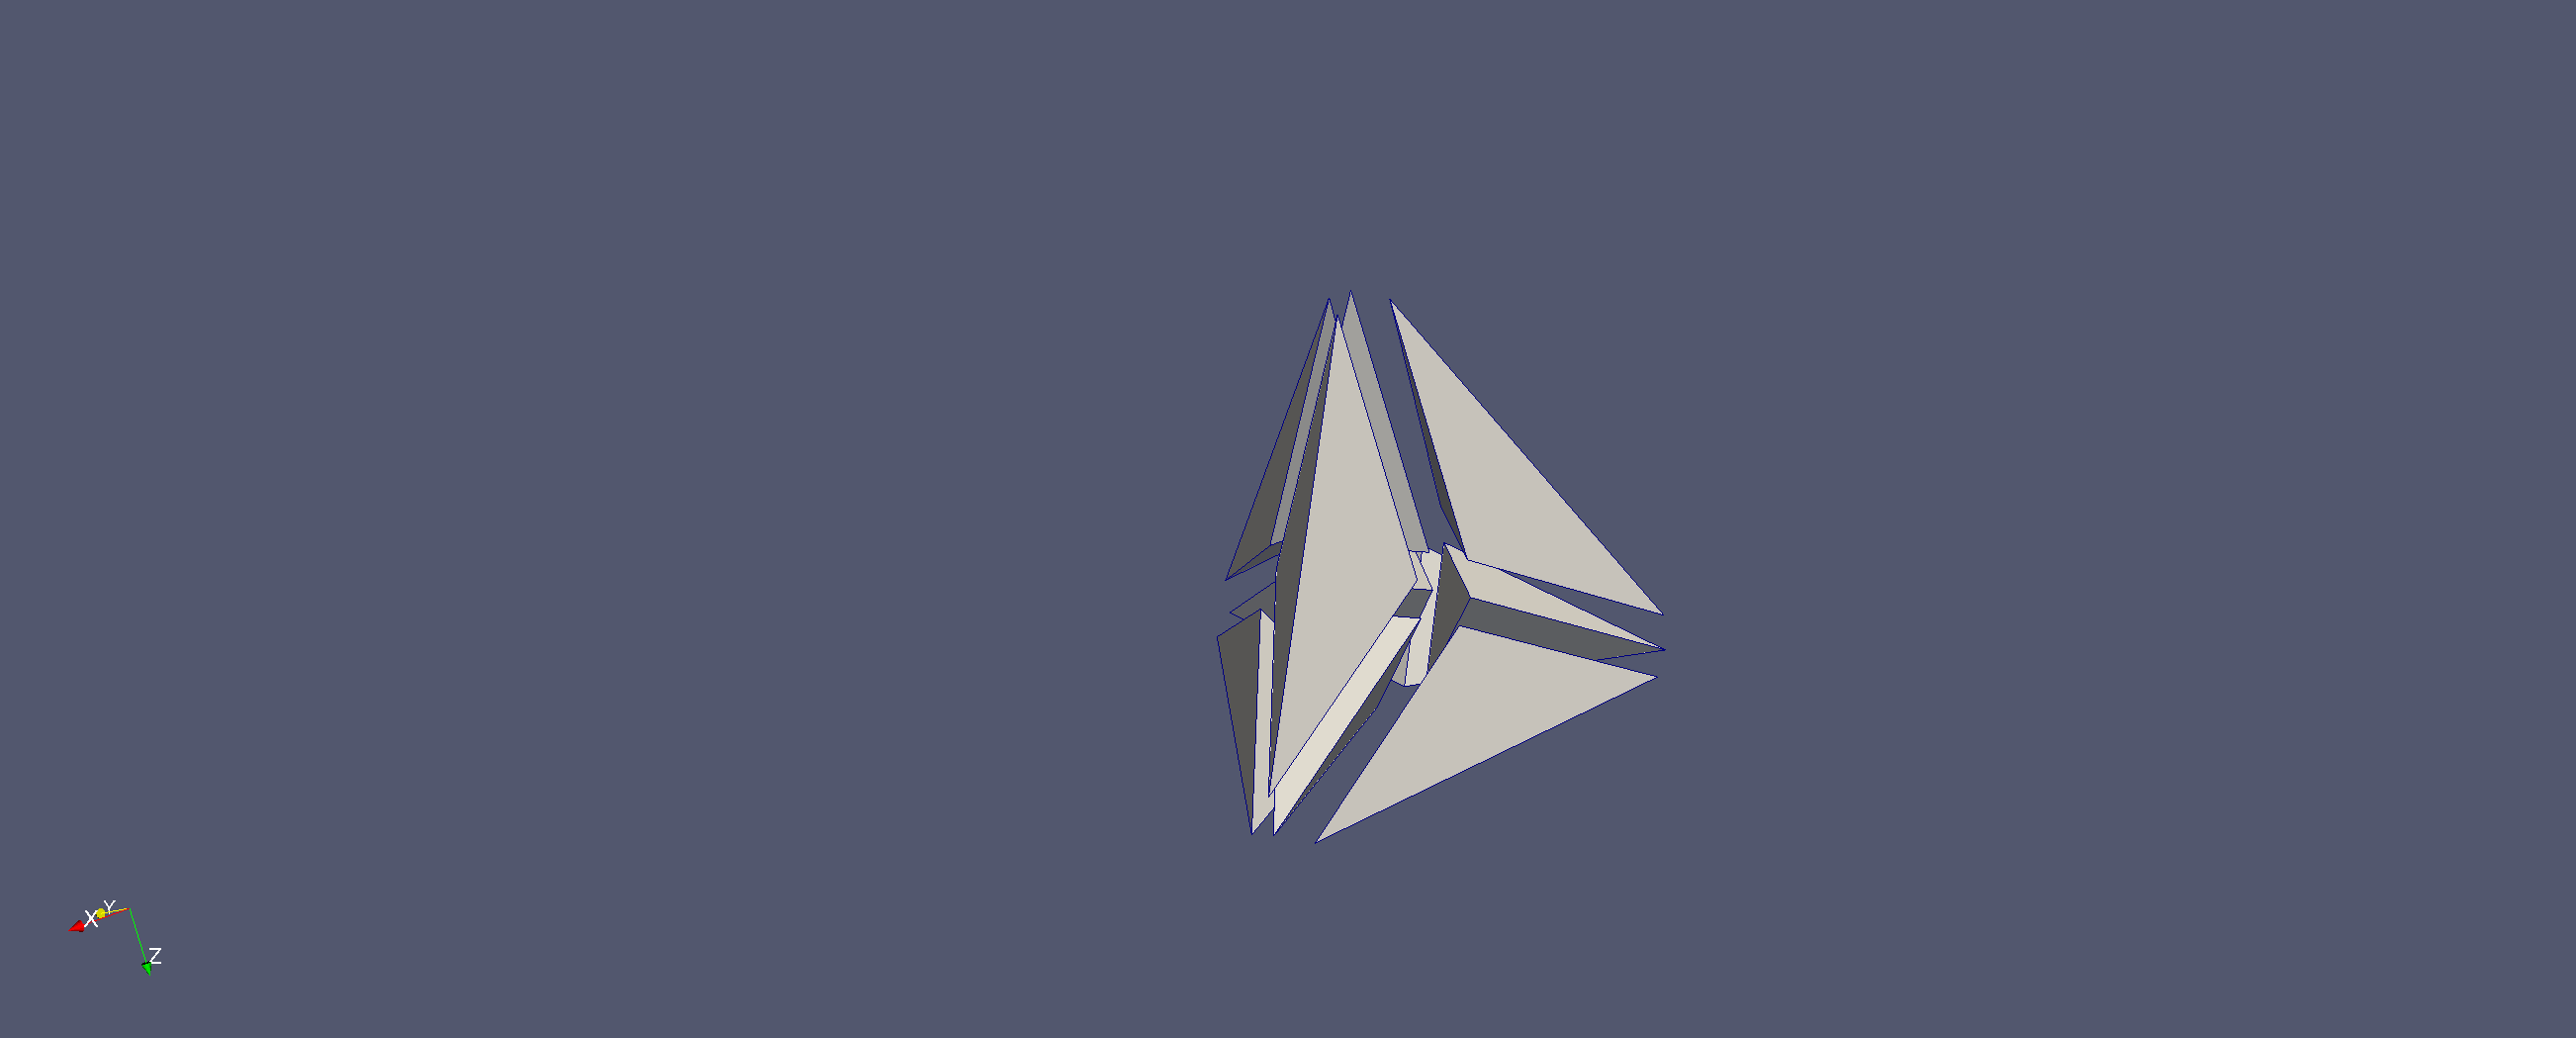
\includegraphics[width=0.85\linewidth]{figures/cutting/Merged_universal.png}
  \caption{---}\label{fig:Merged_universal_subdivision}
\end{figure}

The crack-free subdivision described in the '00 paper (Interactive Simulation of Surgical Cuts) relies on tailored subdivisions for each cut topology. They preserve edges and faces that are uncut, however they introduce the possibility of interpenetrating child tetrahedra. To resolve the issue, geometric checks must be made at runtime and a proper subdivision must be chosen.

\textbf{1 Edge Cut}\\
There are 2 faces that are intact when a single edge of the tetrahedron is cut, and therefore using the modified universal subdivision would leave 2 faces subdivided (needlessly), so we use the crack-free subdivision. This subdivision does not have the issue of interpenetrating child tetrahedra.

\textbf{2 Edges Cut}\\
There are 2 types of 2-edge cut. The first (Type A) is when the cuts are on adjacent edges, that is they share a vertex. The second type (Type B) is when the cuts are not on adjacent edges, they are on edges that are on opposite sides of the tetrahedron.

\textbf{Type A}\\
In this case there is a single face that is uncut, and therefore using the modified universal subdivision is not very well suited. The crack-free subdivision for this cut does not suffer from the interpenetrating child tetrahedra and is therefore suitable for use.

\textbf{Type B}\\
The type B cut is possible to have however is (assumed to be) quite rare. This cut leaves no face uncut on the other hand the crack-free subdivision may present interpenetrating child tetrahedraa, therefore we pick the modified universal subdivision for this case.

\textbf{3 Edges Cut}\\
There are 2 types of 3-edge cut. The first, Type A, is when the 3 cuts are on adjacent edges, and therefore the cut removes the shared vertex, separating the tetrahedra into 2 distinct pieces. The second, Type B, is when the 3 cuts are not adjacent, only one of the cut edges is adjacent to the other two. This cut does not separate the tetrahedron (though may come really close to doing so).

\textbf{Type A}\\
Since all three edges are adjacent, they leave a face uncut, so the modified universal subdivision is not well suited. However, the crack-free subdivision presents the interpenetrating child teterahedra issue. Both subdivisions have issues, but since our priority is to leave untouched edges and faces untouched, we choose the crack-free subdivision, and implement geometry checks in order to pick the proper subdivision. Only a single edge-triangle intersection check is necessary to determine whether the subdivision is valid or not, the edge in question is the one that connects a corner of the tetrahedron to the mid point of its opposite face, while the triangle can be any one of a few faces that get all intersected by the given edge. These triangles are faces of child teterahedra that are independent of the vertices of the edge.

\textbf{Type B}\\
This type cuts all faces and therefore we use the modified universal subdivision since it avoids the geometry checks necessary for the crack-free subdivision.

\textbf{4 Edges Cut}\\
When 4 edges are cut, the tetrahedron is always separated, all faces are cut, and we use the modified universal subdivision to avoid the geometry checks of the crack-free subdivision.

\textbf{Summary of used subdivisions}\\
\begin{table}[]
\begin{tabular}{|l|l|}
\hline
Cut Type     & Subdivision Scheme \\ \hline
1-edge cut   & crack-free         \\ \hline
2-edge cut A & crack-free         \\ \hline
2-edge cut B & modified universal \\ \hline
3-edge cut A & crack-free         \\ \hline
3-edge cut B & modified universal \\ \hline
4-edge cut   & modified universal \\ \hline
\end{tabular}
\caption{--}
\end{table}


\subsection{Types and Composition of Cuts}
From the previous sections we have all the blueprints for subdivisions. In this section we present how the geometry of the cuts are computed based on the tables: using the 1-edge cut and 2-edges cut of type A as base cases, and how we give geometries to the necessary vertices that describe/capture the cut to the tetrahedron. The subdivision comes in to insert child tetrahedra using the new geometries, forming an approximation to the cut tetrahedron.

A tetrahedron may be cut at 0, 1, 2, 3 or 4 edges. To represent a cut configuration each edge is assigned a bit: 0 for uncut, 1 for cut. The ordered sequence of these bits representing the states of the edges is called the bitcode. The respected order of the bitcode is that of the edges given in the earlier section, for example 011001 bitcode represents the cuts at edges 12-20-23 (indicating that the vertex 2 has be split off). When an edge is cut, the virtual vertices involved must be materialized. The tables below describe the exact vertices that need to be materialized, along with some topological information (connectivity, or possible connectivity).

An important aspect of the cutting mechanism is that the information for 1-edge cut and 2-edges cut of type A (1-cut and 2A-cut for short) can be universally used to construct the other types of cuts, in this write-up we call these base cut information or splits. The sharp reader may notice that, for a given bitcode, taking the bitwise OR of the splits produces the corresponding bitcode. This is in general a necessary and sufficient condition for producing the splits of any bitcode into the 1-cut and 2A-cut (not the different between 2A-cut and 2-B cut, type B is produced from from 2 1-cuts on opposing edges, while type A is a base case with 2 edges on a single face).

In summary, the topology of the cut is captured in the bitcode, which is decoded into independent 1-cuts and 2A-cuts that materialize the splitting of the virtual vertices and the subdivision blueprint uses the materialized vertices to insert the child tetrahedron, completing the subdivision of the cut tetrahedron.


\textit{1 Edge cut}
\begin{itemize}
    \item 100000 (01): 4 5
    \item 010000 (12): 6 7
    \item 001000 (20): 8 9
    \item 000100 (03): 10 11
    \item 000010 (13): 12 13
    \item 000001 (23): 14 15
\end{itemize}

\textit{2 Edges cut}\\
\textbf{type A}: the 2 cut edges share a vertex. Two adjacent edges may be cut with or without intersection information on the face they share. In the first case the geometry of the mid face vertices is set using the available information - taking the front weighted average of existing intersections, in the second the geometry is chosen to be a linear interpolation (average) between the edge intersection geometries. In both cases the 4 mid face vertices must be split and assigned to their proper topological sides.

The table below describes the geometric and topological assignments of these vertices. When a face is cut the non-center mid face vertices, of which there are 3, must be split into 1-2. The non-center mid face vertex that is separated from the other 2 is named the loner vertex, while the rest are named group vertices. The center vertex must join either side, giving the topological split cases of '1-3' and '2-2'. Naturally, the '1-3' split is named as such because the center vertex is joined to the group, whereas the '2-2' split is named so because the center vertex joins the loner vertex.

For each bitcode the table indicates the loner vertex and the edge vertices (mid loner) from which its geometry can be derived, similarly the group vertices are listed as well as the edge vertices (mid group) from which their geometry can be derived. The 'summit' column in the table indicates the corner vertex of the tetrahedron that is on the side of the loner relative to the face in question, this helps with quick accessing of geometry checks.

The decision of the '1-3' or '2-2' split is based on the which configuration would yield a none interpenetrating tetrahedra in the subdivision, if one option is valid while the other is not then that option is chosen, if both options are valid, then the one with the best 'curvature' is chosen (the center vertex should go with the convex piece of the split face, the center vertex goes \enquote{against} the curvature of the cut), otherwise the center mid vertex is omitted along with its attached tetrahedron.

Currently this logic is only applied in the case of 4-edges cut with the modified universal subdivision, otherwise the 1-3 split is used as it does not cause any issues with the chosen subdivisions in modified universal non 4-edge cases as the 17th tetrahedron is omitted anyway.


\begin{table}[]
\begin{tabular}{|c|c|c|c|c|c|c|c|}
\hline
bitcode & loner & group  & center & mid loner & mid group & summit & comment \\ \hline
110000  & 17    & 16, 18 & 28     & 5,6       & 4,7       & 1      & 01-12   \\ \hline
101000  & 16    & 18, 17 & 28     & 9,4       & 8,5       & 0      & 01-20   \\ \hline
100100  & 19    & 21, 20 & 29     & 4,10      & 5,11      & 0      & 01-03   \\ \hline
100010  & 21    & 20, 19 & 29     & 12,5      & 13,4      & 1      & 01-13   \\ \hline
011000  & 18    & 17, 16 & 28     & 7,8       & 6,9       & 2      & 12-20   \\ \hline
010010  & 22    & 24, 23 & 30     & 6,12      & 7,13      & 1      & 12-13   \\ \hline
010001  & 24    & 23, 22 & 30     & 14,7      & 15,6      & 2      & 12-23   \\ \hline
001100  & 27    & 26, 25 & 31     & 10,9      & 11,8      & 0      & 20-03   \\ \hline
001001  & 25    & 27, 26 & 31     & 8,14      & 9,15      & 2      & 20-23   \\ \hline
000110  & 20    & 19, 21 & 29     & 11,13     & 10,12     & 3      & 03-13   \\ \hline
000101  & 26    & 25, 27 & 31     & 15,11     & 14,10     & 3      & 03-23   \\ \hline
000011  & 23    & 22, 24 & 30     & 13,15     & 12,14     & 3      & 13-23   \\ \hline
\end{tabular}
\caption{--}
\end{table}
% \caption{Groupings of vertex templates on faces.}







\textbf{type B}: the 2 edges cut do not share a vertex, equivalent to two independent 1-edge cuts, therefore all we need to know is which 1-cut information is required to produce the given bitcode. The table below defines for each bitcode of this type which edges to split open.


\begin{table}[]
\begin{tabular}{|l|l|l|l|}
\hline
bitcode & split 1      & split 2        & comment \\ \hline
100001  & 100000 (4,5) & 000001 (14,15) & 01-23   \\ \hline
010100  & 010000 (6,7) & 000100 (10,11) & 12-03   \\ \hline
001010  & 001000 (9,8) & 000010 (12,13) & 20-13   \\ \hline
\end{tabular}
\caption{--}
\end{table}




\textit{3 Edges cut}\\
\textbf{type A}: the 3 edges cut share a vertex cutting it off from the main tetrahedron. These can be solved by independently applying the single edge split on the three edges that are connected to the vertex, and then applying three 2A-cuts on each involved face, each of which is based on the newly created edge splits. The first table gives, for each bitcode, the edges that need to be split, the second table gives the faces that need to be split. The table of edges is very straightforward as every '1' in the bitcode is translated to an edge to split, the table of faces is a bit more involved since it requires all pairs (in this case) of '1' bitcode splits.

(edge)\\
\begin{table}[]
\begin{tabular}{|l|l|l|l|l|}
\hline
bitcode & split 1        & split 2        & split 3        & comment    \\ \hline
110010  & 100000 (4,5)   & 010000 (6,7)   & 000010 (12,13) & cuts off 2 \\ \hline
101100  & 100000 (4,5)   & 001000 (9,8)   & 000100 (10,11) & cuts off 0 \\ \hline
011001  & 010000 (6,7)   & 001000 (9,8)   & 000001 (14,15) & cuts off 3 \\ \hline
000111  & 000100 (10,11) & 000010 (12,13) & 000001 (14,15) & cuts off 1 \\ \hline
\end{tabular}
\caption{--}
\end{table}
% \caption{Edge table for 3 Edges type A cut showing the cut edge components.}


(face)\\
\begin{table}[]
\begin{tabular}{|l|l|l|l|l|}
\hline
bitcode & face 1 & face 2 & face 3 & comment    \\ \hline
110010  & 110000 & 010010 & 100010 & cuts off 2 \\ \hline
101100  & 101000 & 100100 & 001100 & cuts off 0 \\ \hline
011001  & 011000 & 010001 & 001001 & cuts off 3 \\ \hline
000111  & 000110 & 000101 & 000011 & cuts off 1 \\ \hline
\end{tabular}
\caption{--}
\end{table}
% \caption{Face table for 3 Edges type A cut showing the cut face components.}


\textbf{type B}: the 3 edges cut do not share a vertex, 2 adjacent faces are cut at 2 of their edges. This can be solved rather similarly to type A, by first applying the 1-cut splits, then applying only two 2A-cuts on the involved faces. The tables are constructed similarly to their type A counterpart.

(edge)\\
\begin{table}[]
\begin{tabular}{|l|l|l|l|l|}
\hline
bitcode & split 1 & split 2 & split 3 & comment \\ \hline
110100  & 100000  & 010000  & 000100  &         \\ \hline
110001  & 100000  & 010000  & 000001  &         \\ \hline
101010  & 100000  & 001000  & 000010  &         \\ \hline
101001  & 100000  & 001000  & 000001  &         \\ \hline
100101  & 100000  & 000100  & 000001  &         \\ \hline
100011  & 100000  & 000010  & 000001  &         \\ \hline
011100  & 010000  & 001000  & 000100  &         \\ \hline
011010  & 010000  & 001000  & 000010  &         \\ \hline
010110  & 010000  & 000100  & 000010  &         \\ \hline
010101  & 010000  & 000100  & 000001  &         \\ \hline
001110  & 001000  & 000100  & 000010  &         \\ \hline
001011  & 001000  & 000010  & 000001  &         \\ \hline
\end{tabular}
\caption{--}
\end{table}
% \caption{Edge table for 3 Edges type B cut showing the cut edge components.}

(face)\\
\begin{table}[]
\begin{tabular}{|l|l|l|l|}
\hline
bitcode & face 1 & face 2 & comment \\ \hline
110100  & 110000 & 100100 &         \\ \hline
110001  & 110000 & 010001 &         \\ \hline
101010  & 101000 & 100010 &         \\ \hline
101001  & 101000 & 001001 &         \\ \hline
100101  & 100100 & 000101 &         \\ \hline
100011  & 100010 & 000011 &         \\ \hline
011100  & 011000 & 001100 &         \\ \hline
011010  & 011000 & 010010 &         \\ \hline
010110  & 010010 & 000110 &         \\ \hline
010101  & 010001 & 000101 &         \\ \hline
001110  & 001100 & 000110 &         \\ \hline
001011  & 001001 & 000011 &         \\ \hline
\end{tabular}
\caption{--}
\end{table}
% \caption{Face table for 3 Edges type B cut showing the cut face components.}


Note that the middle tetrahedron is not inserted in this subdivision, for visual fidelity. This results in a 1-to-16 subdivision. The deletion of the 17th tetrahedron is not necessary, however it requires a very involved handcrafting of the conditions for each of the 12 cases.


disallowed cuts: these cuts are not allowed since they cut all three edges of a single face, which is not supposed to happen with a single cut segment. These can happen with a sequence of cut segments that are taken to be a single cut, however to get this bit code from a single such cut is rare since it involves very sharp turns, so if it happens, one could handle it by dividing the sequence into parts and applying the parts in order.


\begin{table}[]
\begin{tabular}{|l|l|}
\hline
bitcode & comment  \\ \hline
111000  & face 012 \\ \hline
100110  & face 031 \\ \hline
010011  & face 132 \\ \hline
001101  & face 230 \\ \hline
\end{tabular}
\caption{--}
\end{table}



\textit{4 Edges cut}\\
These can be solved by applying four 1-cuts then four 2A-cuts, the tables follow their counterparts of the 3-edges cut.

(edge)\\
\begin{table}[h]
\begin{tabular}{|l|l|l|l|l|l|}
\hline
bitcode & split 1 & split 2 & split 3 & split 4 & comment \\ \hline
110101  & 100000  & 010000  & 000100  & 000001  &         \\ \hline
011110  & 010000  & 001000  & 000100  & 000010  &         \\ \hline
101011  & 100000  & 001000  & 000010  & 000001  &         \\ \hline
\end{tabular}
\caption{--}
\end{table}
% \caption{Edge table for 4 Edges cut showing the cut edge components.}



(face)\\
\begin{table}[h]
\begin{tabular}{|l|l|l|l|l|l|}
\hline
bitcode & face 1 & face 2 & face 3 & face 4 & comment \\ \hline
110101  & 110000 & 100100 & 010001 & 000101 &         \\ \hline
011110  & 011000 & 010010 & 001100 & 000110 &         \\ \hline
101011  & 101000 & 100010 & 001001 & 000011 &         \\ \hline
\end{tabular}
\caption{--}
\end{table}
% \caption{Face table for 4 Edges cut showing the cut face components.}




Note that, when 4 edges are cut, the central tetrahedron has $2^4$ possible topological configurations: each of its vertices may be on one or the other of the separated pieces of the original tetrahedron (). There are of course only 2 valid configurations as the tetrahedron must be completely attached to only one of the pieces of the split tetrahedron, in addition to the possibility of just not adding it.

The correct decision requires the steps listed in the 2-edges cut type A, to check for interpenetrating tetrahedra for the different possible configurations and deciding based on the geometry of the cut.

\subsection{Cutting Algorithm}
\subsubsection{Core Cutting}

The core cutting algorithms are encapsulated in the CuttingSystem abstraction. The CuttingSystem defines a clean public interface to the cutting mechanism through primarily two cutting methods: one cut and progressive cut. One cut is used when the full cut geometry is known while progressive cut deals with a continuous cut where the cut geometry is not predefined. These methods have guards to prevent any false starts and to ensure proper termination of the procedure. Figure \ref{fig:Cutting_process_flow} shows the flow for the progressive cut.

Both methods are similar in that they invoke BVH intersection method when given cut geometry in the form of triangles approximating the cut surface and segments describing the movement of certain points of the tool. The BVH intersection computation is fast and global. Unlike Bielser’s approach of local (topological) propagation of the cut, the BVH approach allows cutting disconnected parts of a mesh. \ref{fig:BVH_flow}

The intersection information on the edges and faces is used to determine which cells were affected, and in the case of progressive cut, which cells are active, that is the cells that are pierced by the last position of the cutting tool. The active cells are treated differently as their subdivision is not yet complete in the mesh as a subsequent movement of the tool could cut the cell further and cause an internal topology change, handled by the state machine introduced by Bielser. With the intersections completed the cut can be processed. Subdivision can take place and the resulting changes are reported back to the BVH to update its internal structure, and the physics engine to let it know of new vertices and edges that need to be accounted for.

Processing of the cut distinguishes between finalized and active cells, where finalized cells are affected cells that are not active. Each is treated differently primarily because the resulting changes to the mesh need to be treated differently. BVH deals only with the part of the mesh that is possible to intersect, therefore the changes resulting from active cells should not be reported to it. On the other hand, physics should be aware of the exact state of the mesh topology, therefore everything is reported to it. To keep track of the affected, active, finalized cells as well as their children a CutTetrahedronManager object is used to provide all the management functionalities.\ref{fig:Process_cut_details_flow}

Each cell is treated independently. If there is no topology change to the cell, its geometry (its children’s geometry) is updated. Otherwise, the cell gets a first or a new subdivision once the new vertices are determined and set in the mesh. The subdivision process itself is very involved and another point where this work diverges from Bielser’s. First a modified universal subdivision is introduced that merges cells along uncut edges. This does not eliminate “crack”s in the mesh, however in the select cases where it is used, it ensures that uncut edges are not subdivided. We also use the cut-specific subdivisions. The use cases are shown in the subdivision diagram level 3. This mix of subdivision ensures the fewest the introduction of fewer cells, a major drawback of any subdivision based geometry cutting. \ref{fig:CutTetrahedron_flow} \ref{fig:Subdivision_flow}


\begin{figure}
  \centering%
  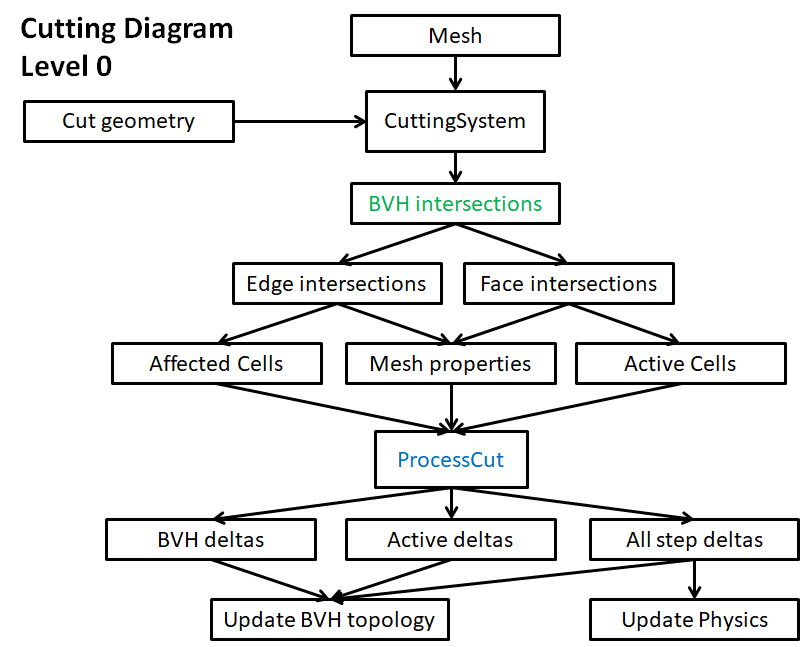
\includegraphics[width=0.85\linewidth]{figures/cutting/Process_cut.png}
  \caption{---}\label{fig:Cutting_process_flow}
\end{figure}



\begin{figure}
  \centering%
  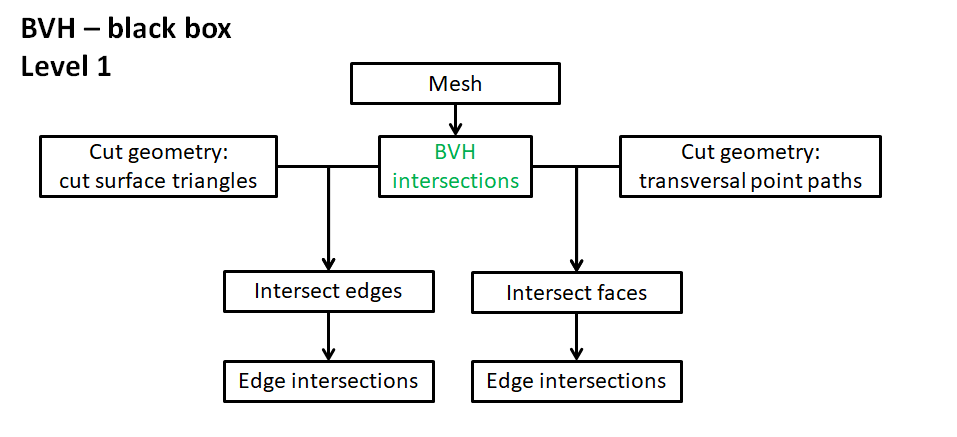
\includegraphics[width=0.85\linewidth]{figures/cutting/BVH.png}
  \caption{---}\label{fig:BVH_flow}
\end{figure}


\begin{figure}
  \centering%
  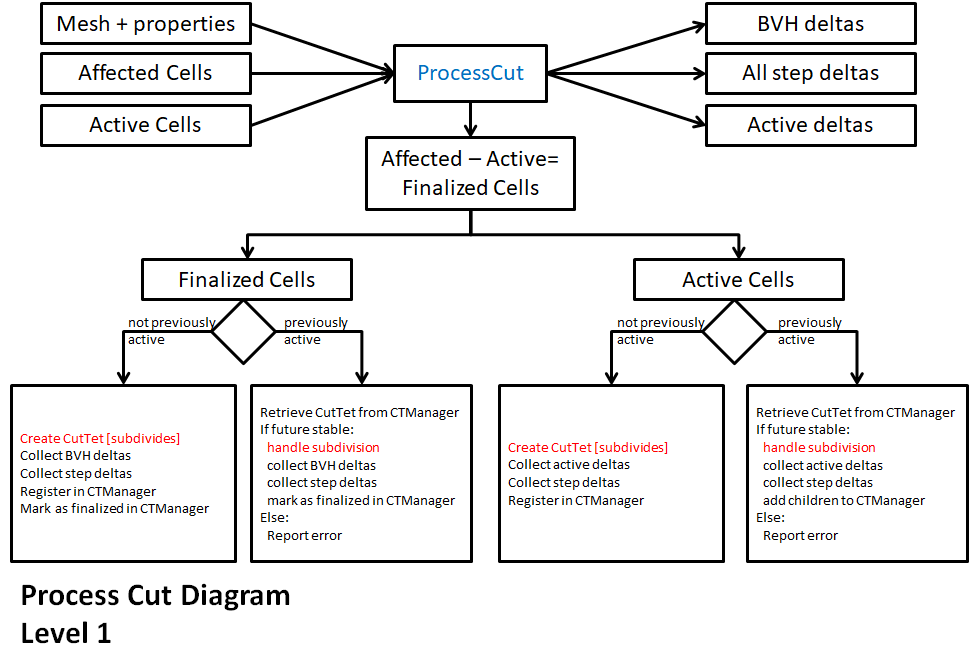
\includegraphics[width=0.85\linewidth]{figures/cutting/Process_cut_details.png}
  \caption{---}\label{fig:Process_cut_details_flow}
\end{figure}


\begin{figure}
  \centering%
  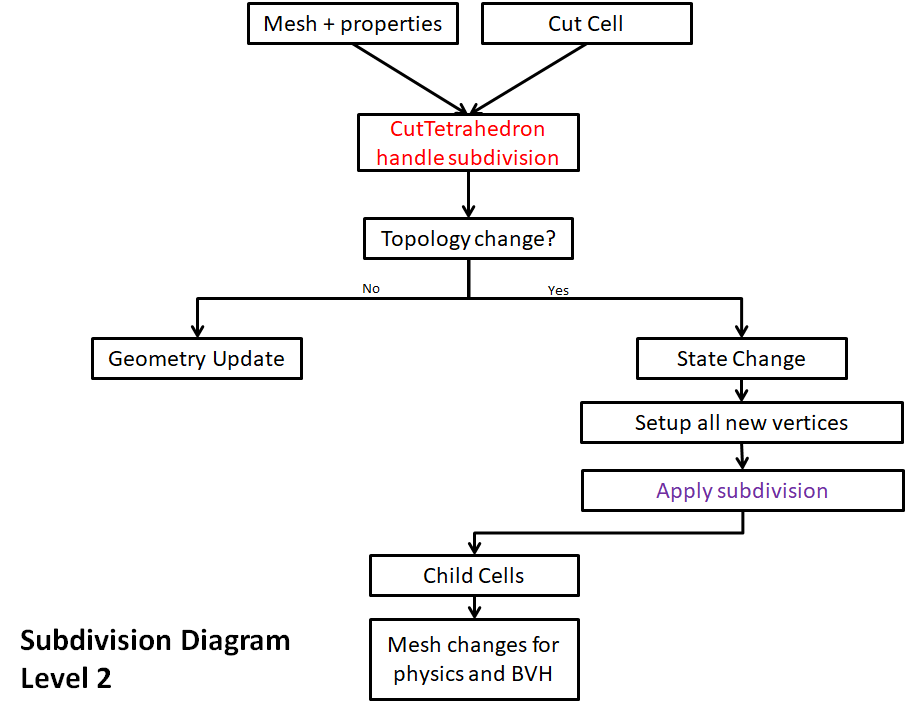
\includegraphics[width=0.85\linewidth]{figures/cutting/cuttetrahedron.png}
  \caption{---}\label{fig:CutTetrahedron_flow}
\end{figure}


\begin{figure}
  \centering%
  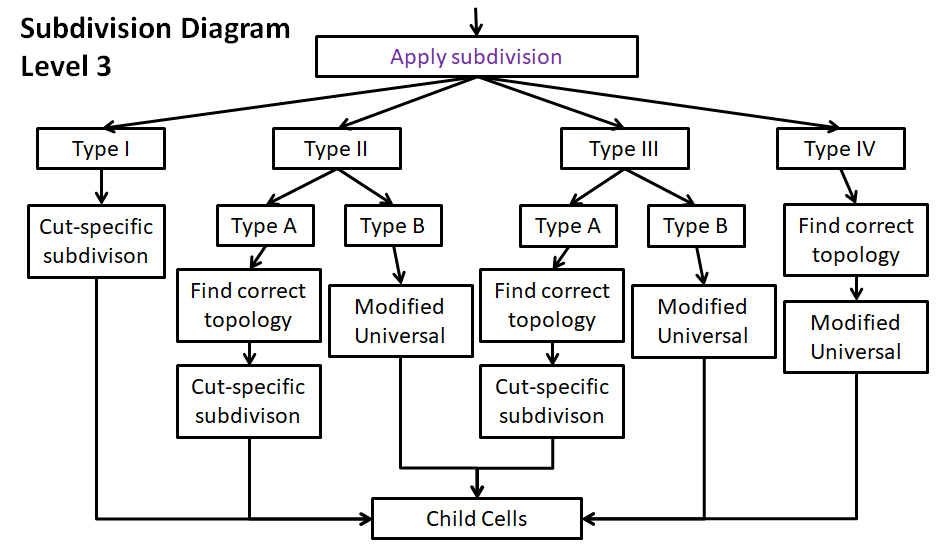
\includegraphics[width=0.85\linewidth]{figures/cutting/subdivision.png}
  \caption{---}\label{fig:Subdivision_flow}
\end{figure}


\subsubsection{Enhanced Cutting Operations}

\textbf{Adaptive Cutting}\\

\textbf{Mesh Cleanup and Simplification}\\
Once the cut is processed and the mesh updates are done, a further post-process first cleans the mesh of any flat cells and reduces the number of new cells. The mesh simplification algorithm maintains a good mesh topology without cell inversions, a problem that is usually hard to solve globally, it also maintains the geometry of the cut on the mesh as well as the mesh volume for maximum visual fidelity on all levels.

The algorithm operates by iterating on edge contractions. An edge contraction operation on edge $ij$ removes vertex $j$ and reattaches to $i$ all tetrahedra that were incident to $j$. Edge contraction follows an order based on the priority of vertices. Vertices on the cutting surface are of highest priority and are not removed in order to preserve the shape of the cut. Vertices in the interior of the volume have lowest priority and are removed first to simplify the mesh. Vertices on the boundary are next in the priority and are removed as needed to simplify the model while keeping the original volume intact.

\clearpage

\section{Scalable Methods for Non-linear Real-time Finite Element Simulation}\label{sec:fem_simulation}

\subsection{Incremental Introduction of Cuts and Discontinuities in 3D meshes}\label{ssec:discontinuous_fem}
One modeling challenge in surgical simulation is the geometric and topological representation of cuts and their effects on an underlying tetrahedral mesh. Data structures and algorithms to address this problem are described next. 

\subsubsection{Tetrahedral Subdivision Template}

Cutting a tetrahedral mesh should result in a new mesh retaining topological integrity in addition to exhibiting the cut geometrically. In order to capture general cut topologies, a tetrahedral subdivision scheme with the granularity to represent various types of topological cuts is needed. To this end we built a generic 32-vertex tetrahedral template, where arrangements of these vertices can generate the various discontinuities that appear during cutting. 

\begin{figure}
	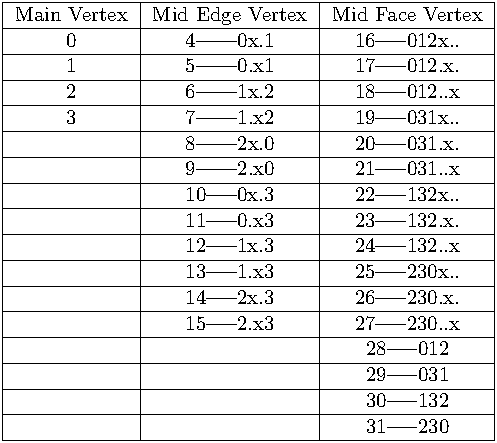
\includegraphics[width=0.6\textwidth]{cutting/vertextable.pdf}
	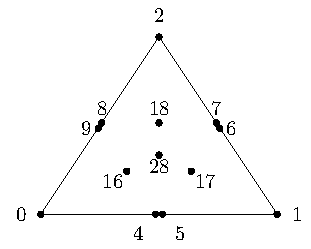
\includegraphics[width=0.4\textwidth]{cutting/face.pdf}
	\caption{Vertices in the subdivision template. The vertices on face 012 are shown on the right.}
	\label{fig:vertices}
\end{figure}

Figure \ref{fig:vertices} lists the 32 virtual vertices on the surface of the template sudivision tetrahedron. These vertices are distinct only topologically, not geometrically. The table lists these vertices in three categories: vertices of the original tetrahedron, vertices at the middle of edges, and vertices at the middle of faces. For the subdivision, an edge is split into 2, requiring 2 vertices in the (topological) middle of the edge. A face is split into 4 or 5 triangles and requires 4 vertices in the (topological) middle of the face. The notation used in the table is as follows. The mid-edge vertex $i\times .j$ denote the vertex on edge $ij$ closest to $i$. The mid-face $ijk\times ..$ denotes the vertex on face $ijk$ closest to the position denoted by the $\times$. The vertex denoted as $ijk$ is the mid-face vertex on face $ijk$. 

Assuming that cuts are limited to a single cut per edge and no more than 2 cuts on the edges of a triangular face, 
these vertices provide the necessary topology for a tetrahedron to be properly subdivided into 17 children tetrahedra. However these subdivisions may be produce incompatible meshes where an edge or face may be subdivided differently depending on the tetrahedra it is connected to. These incompatible subdivisions produce hanging nodes that complicate the physical simulation. In order to avoid these incompatibilities in the mesh, the generic subdivision is modified to merge the children tetrahedra that lie on a single undivided edge. This reduces the number of child tetrahedra and as importantly preserves a full connectivity with neighbors sharing uncut edges. The resulting subdivision template is shown in Figure \ref{fig:Merged_universal_subdivision}. In addition, subdivided faces with uncut edges are also merged to avoid face cracks between neighboring tetrahedra. 

\begin{figure}
  \centering%
  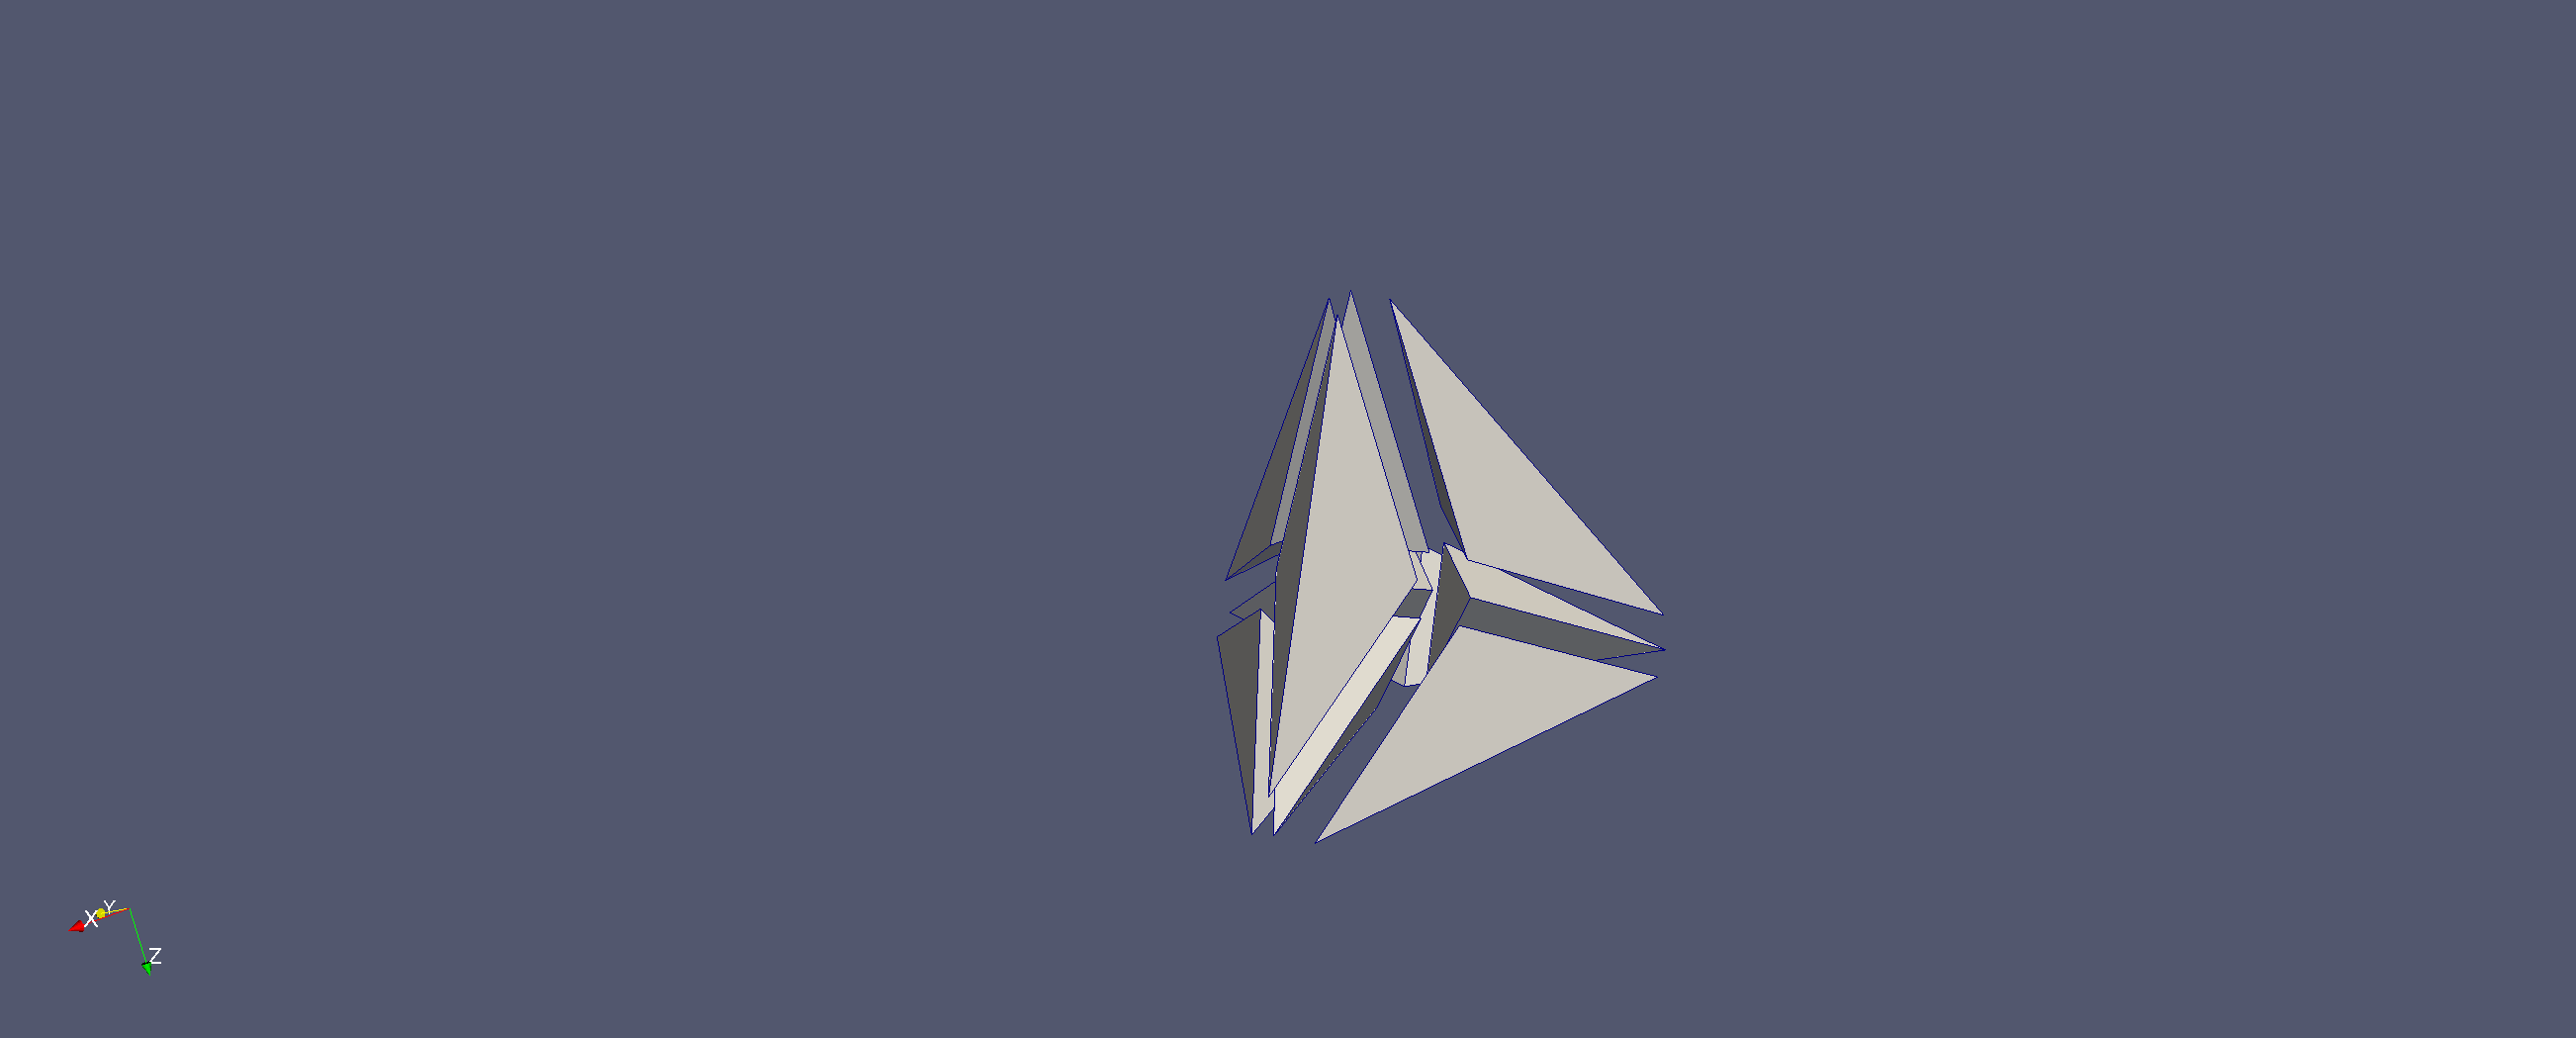
\includegraphics[width=0.85\linewidth]{figures/cutting/Merged_universal.png}
  \caption{Universal subdivision tetrahedral template with merged children along edges.}\label{fig:Merged_universal_subdivision}
\end{figure}


\subsubsection{Types of Subdivision}

The template above supports the five types of topologically-distinct discontinuous tetrahedral elements that occur during incision. The top portion of \autoref{fig:discontinuous_tetrahedra_fem} shows the 1-edge, 2-edge, and 3-edge cases (involving edges sharing a vertex), while the left two pictures of the bottom portion show the 3-edge and 4-edge cases (involving edges around two different vertices). These elements involve planar cuts inside individual elements. A complete cut with compatibility between neighbors is shown on the right of the bottom row.

\begin{figure}
  \centering%
  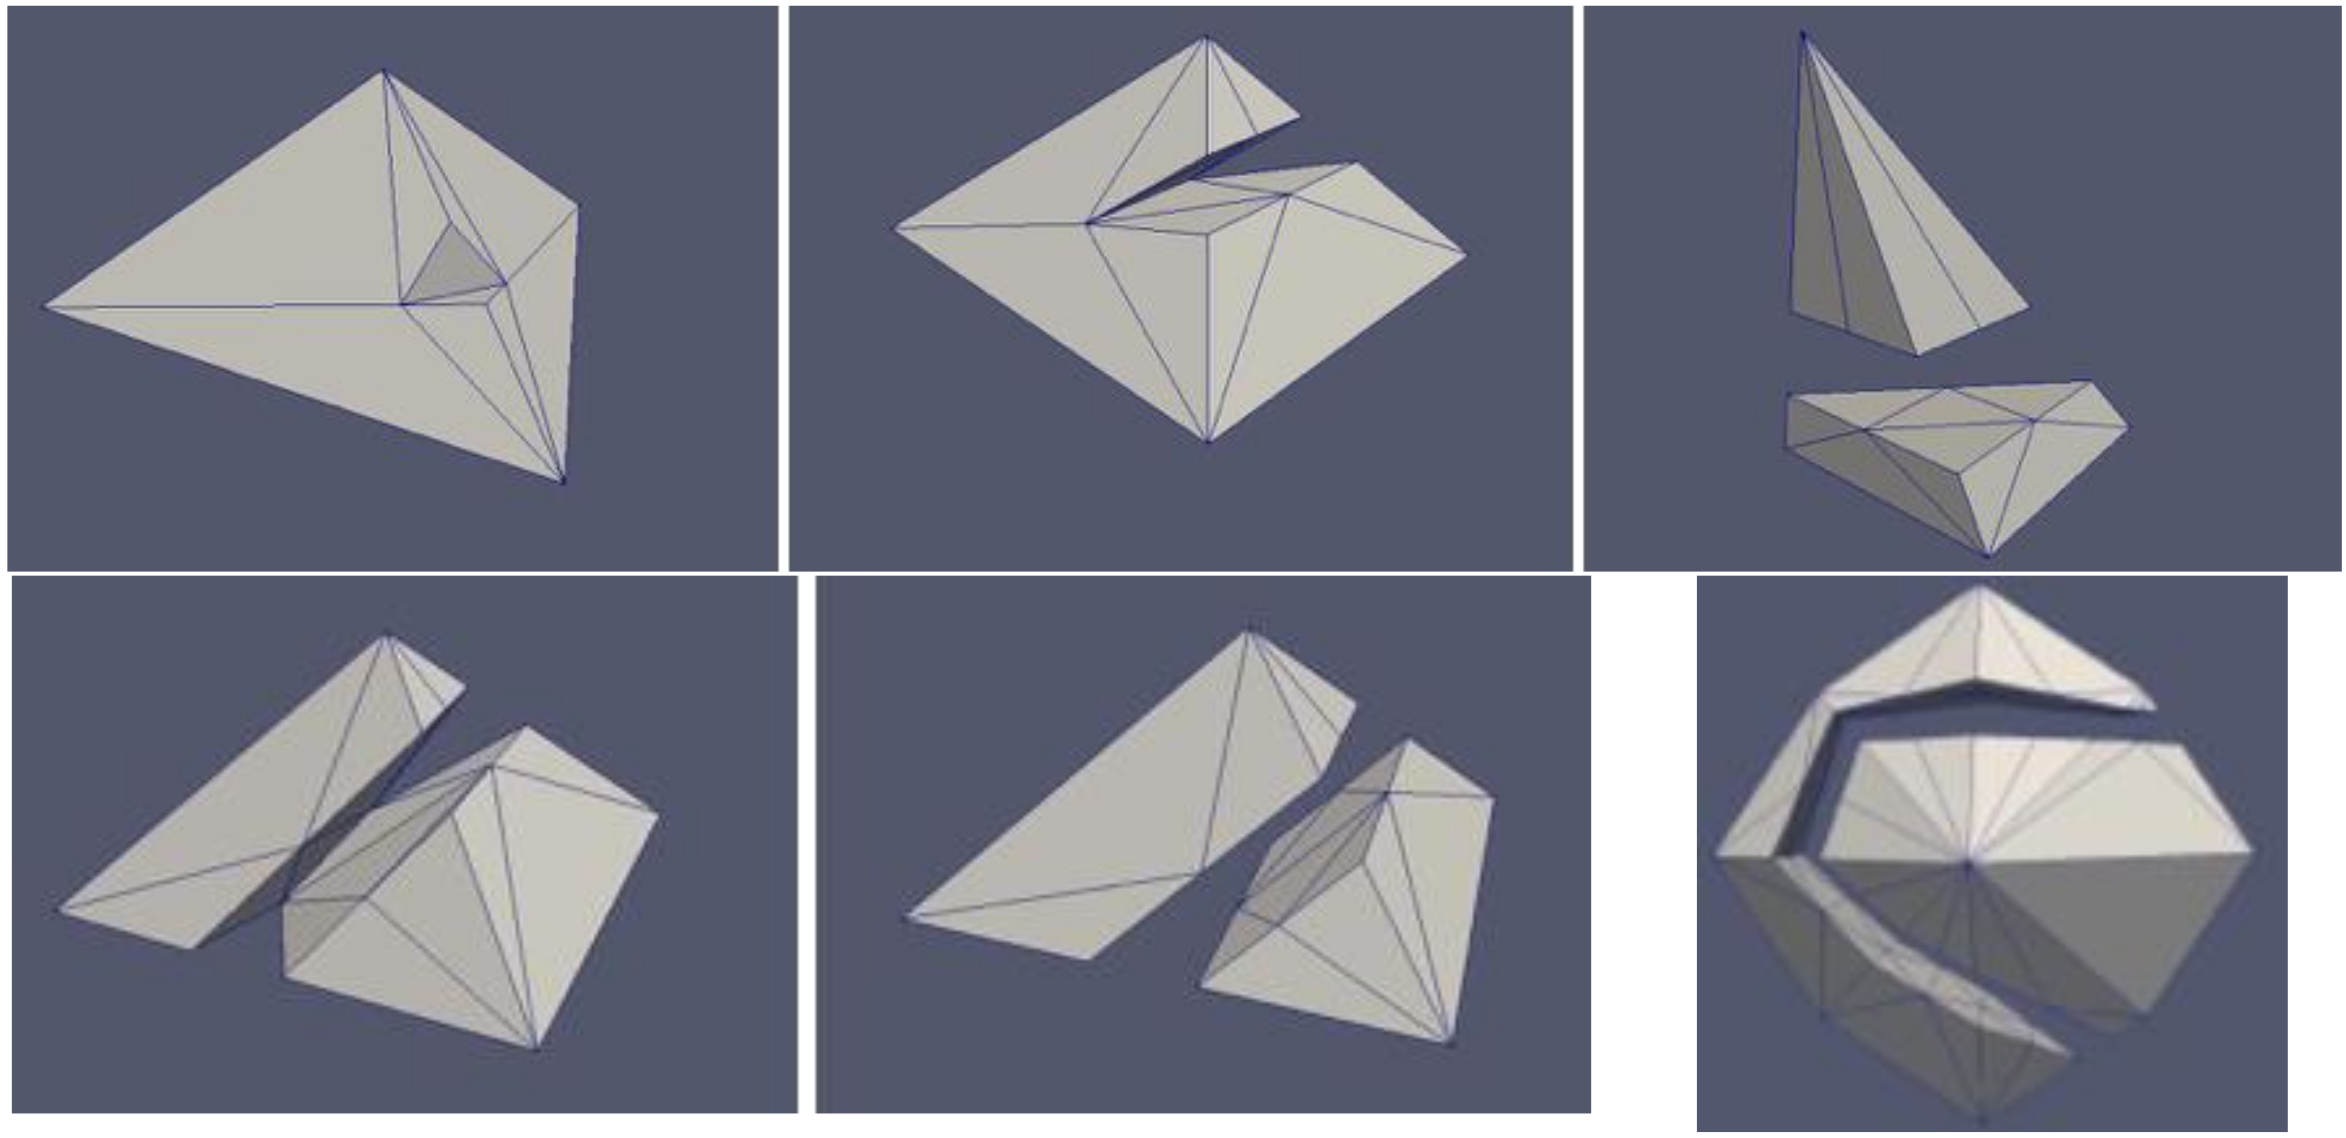
\includegraphics[width=0.85\linewidth]{simulation/cut_configurations}
  \caption{---}\label{fig:discontinuous_tetrahedra_fem}
\end{figure}


One of the challenges of robust cutting is the case of edges that get cut twice. This occurs when tool paths with extensive curvature take place. This configuration is not directly supported by the subdivision template above, and an adaptive refinement of the mesh is needed. We developed a procedure that automatically refines the mesh when a doubly cut edge is encountered. The refinement divides the tetrahedra incident in this edge in such a way as to be able to apply the regular subdivision on the resulting mesh.  An example of this adaptive cut-aware refinement is shown in \autoref{fig:tet_cuts}.

\begin{figure}
  %\captionsetup[subfigure]{width=0.2\textwidth}
  \centering%
  \subbottom[]{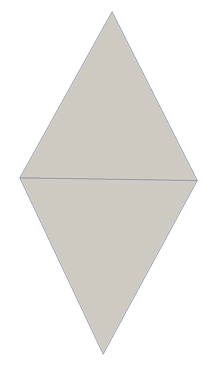
\includegraphics[width=0.19\textwidth]{simulation/tet_cut1}\label{fig:tet_cut1}}
  \hfill%
  \subbottom[]{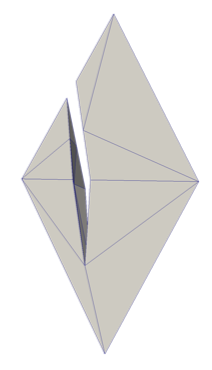
\includegraphics[width=0.19\textwidth]{simulation/tet_cut2}\label{fig:tet_cut2}}
  \hfill%
  \subbottom[]{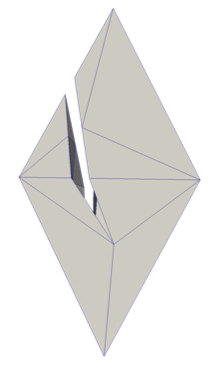
\includegraphics[width=0.19\textwidth]{simulation/tet_cut3}\label{fig:tet_cut3}}
  \hfill%
  \subbottom[]{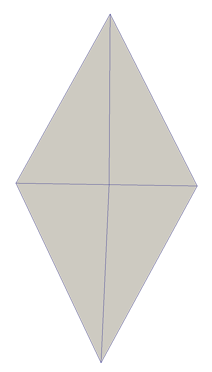
\includegraphics[width=0.19\textwidth]{simulation/tet_cut4}\label{fig:tet_cut4}}
  \hfill%
  \subbottom[]{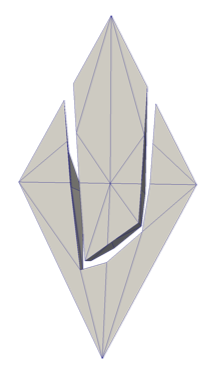
\includegraphics[width=0.19\textwidth]{simulation/tet_cut5}\label{fig:tet_cut5}}
  \caption{This figure shows 2 tetrahedra (\emph{a}), top and bottom, and a cut that intersects an edge separating the 2 tetrahedra (\emph{b}) curves inside the bottom one (\emph{c}) and exits intersecting the same edge. When the second cut is detected, the mesh is refined as seen in (\emph{d}), and the cut reapplied (\emph{e}).}\label{fig:tet_cuts}
\end{figure}


Finally, the subdivision scheme could result under certain conditions in some flat tetrahedra. A post-process is used to clean the mesh from such anomalies. An example is shown in \autoref{fig:flat_tet}. This post-process, that follows the introduction of an incision, is also used to improve mesh quality by removing tetrahedra with poor shapes and aspect ratios. This mesh simplification algorithm operates by iterating on edge contractions. An edge contraction operation on edge $ij$ removes vertex $j$ and reattaches to $i$ all tetrahedra that were incident to $j$. Edge contraction follows an order based on the priority of vertices. Vertices on the cutting surface path are of highest priority and are not removed in order to preserve the shape of the cut. Vertices in the interior of the volume have lowest priority and are removed first to simplify the mesh. Vertices on the boundary are next in the priority and are removed as needed to simplify the model while keeping the original volume intact.


\begin{figure}
  \centering%
  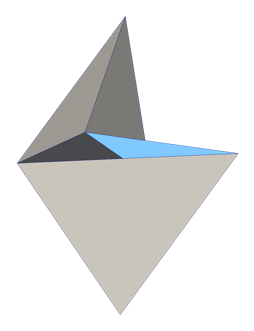
\includegraphics[width=0.3\textwidth]{simulation/tet_flat1}\label{fig:tet_flat1}
  \hspace{10ex}
  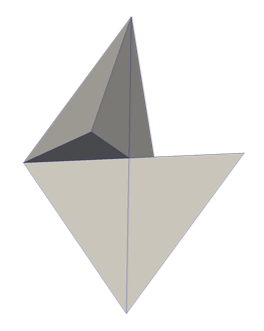
\includegraphics[width=0.3\textwidth]{simulation/tet_flat2}\label{fig:tet_flat2}
  \caption{In this figure, the left mesh (3 tetrahedra) admits a single flat cell shaded in blue, on the right the cluster of affected cells are removed and replaced with an equivalent set (4 tetrahedra) without any flat cells.}\label{fig:flat_tet}
\end{figure}

% In the Figure, the left mesh (3 tetrahedra) admits a single flat cell shaded in blue, on the right the cluster of affected cells are removed and replaced with an equivalent set (4 tetrahedra) without any flat cells.

% This task is now complete and has been tested on a variety of configurations. The system has the ability to handle a variety of cutting scenarios that introduce different topological configurations of the cut tetrahedra. Different parameters allow the system to handle different physical parameters, involving more or less or more prestress in the material, as well as different geometric configurations. The figure below includes illustrations of discontinuities introduced in volumetric tetrahedral meshes.  When cuts are introduced, edges may be cut twice requiring additional adaptive tetrahedral refinements that are handled by the system transparently.

These subdivision methods have the ability to handle in a robust manner a variety of cutting scenarios that introduce different topological configurations of the cut tetrahedra. \autoref{fig:cuts} below includes illustrations of discontinuities introduced in volumetric tetrahedral meshes.  When cuts are introduced, edges may be cut twice requiring additional adaptive tetrahedral refinements that are handled by the system transparently.

\begin{figure}
  \centering%
  \setlength{\fboxsep}{0pt}%
  \setlength{\fboxrule}{0.1pt}%
  \fbox{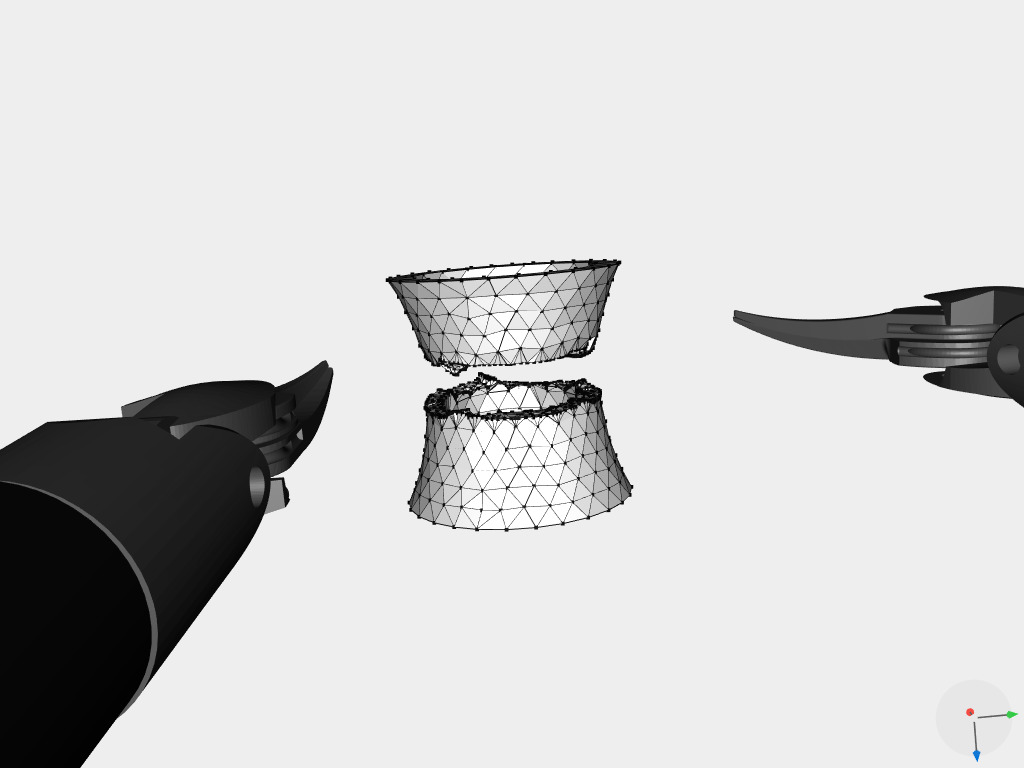
\includegraphics[width=0.32\linewidth]{simulation/snip0}}
  \hfill%
  \fbox{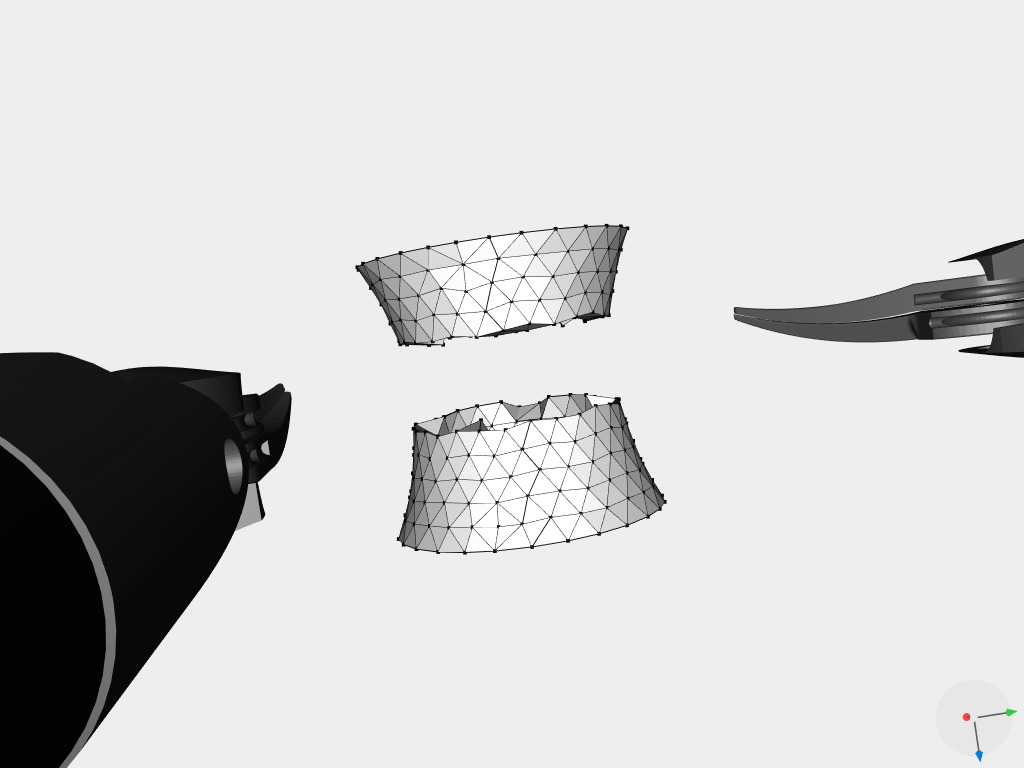
\includegraphics[width=0.32\linewidth]{simulation/snip1}}
  \hfill%
  \fbox{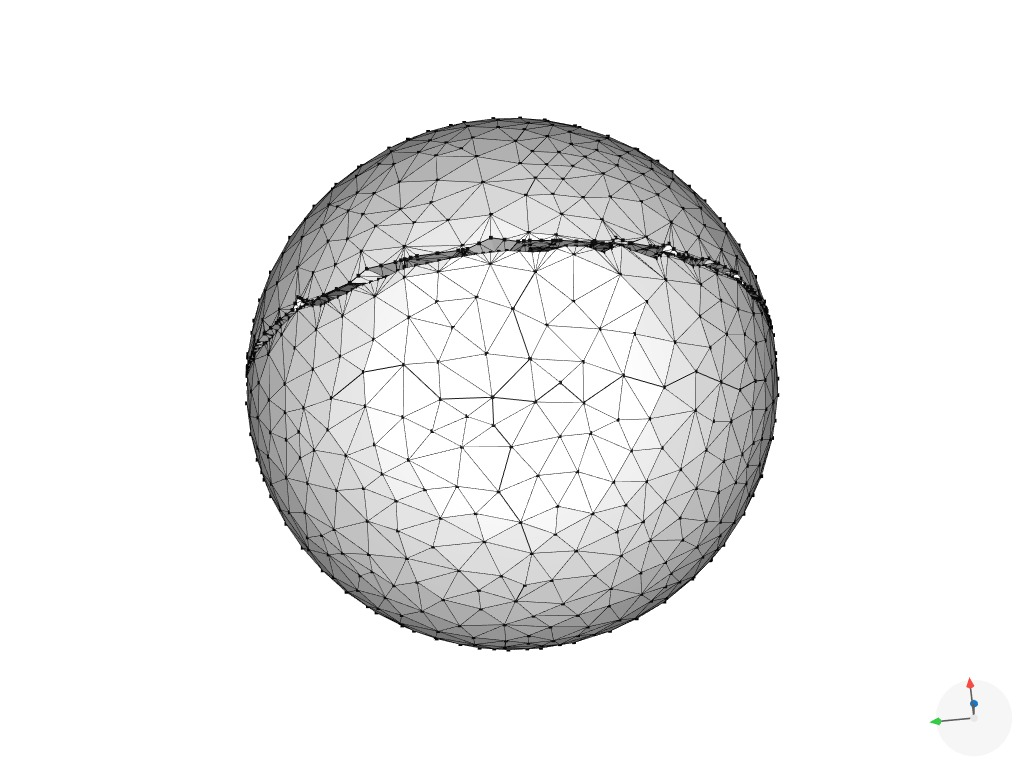
\includegraphics[width=0.32\linewidth]{simulation/snip2}}
  \caption{---}\label{fig:cuts}
\end{figure}

% ======================================================================

\clearpage
\subsection{Fast Incremental Solver}\label{ssec:incremental_solver}

% \subsubsection{Incremental Cutting Architecture}

\autoref{fig:Cutting_process_flow} shows the overall flow of the progressive cutting procedure. The first step in the procedure is to compute intersections of the tool surface path with the edges and faces of the mesh. A Bounding Volume Hierarchy (BVH) data structure is used to allow for fast computations of global intersections allowing disconnected parts of the mesh to be cut as the cutting tool is swept. The intersection information on the edges and faces is used to determine which tetrahedral cells are affected and which are active. Affected cells are those that have been intersected by the tool path and active cells are those pierced by the last position of the cutting tool. The active cells are treated differently than others as their subdivision is not yet complete in the mesh as a subsequent movement of the tool could cut the cell further and cause an internal topology change.  When the intersections are completed, the cut can be processed. Subdivision can then take place and the resulting changes are reported back to the BVH to update its internal structure, and to the finite element (FE) physics engine to communicate new and deleted vertices and edges.  

\begin{figure}
  \centering%
  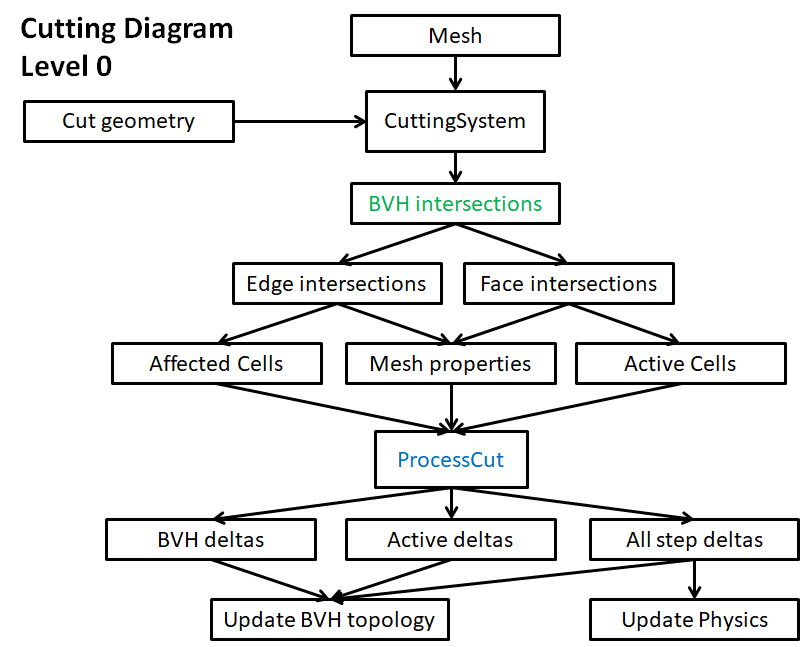
\includegraphics[width=0.75\linewidth]{figures/cutting/Process_cut.png}
  \caption{Flow of progressive cutting procedure.}\label{fig:Cutting_process_flow}
\end{figure}



% Processing of the cut distinguishes between finalized and active cells, where finalized cells are affected cells that are not active. Each is treated differently primarily because the resulting changes to the mesh need to be treated differently. BVH deals only with the part of the mesh that is possible to intersect, therefore the changes resulting from active cells should not be reported to it. On the other hand, physics should be aware of the exact state of the mesh topology, therefore everything is reported to it. To keep track of the affected, active, finalized cells as well as their children a CutTetrahedronManager object is used to provide all the management functionalities.\ref{fig:Process_cut_details_flow}

% Each cell is treated independently. If there is no topology change to the cell, its geometry (its children’s geometry) is updated. Otherwise, the cell gets a first or a new subdivision once the new vertices are determined and set in the mesh. The subdivision process itself is very involved and another point where this work diverges from Bielser’s. First a modified universal subdivision is introduced that merges cells along uncut edges. This does not eliminate “crack”s in the mesh, however in the select cases where it is used, it ensures that uncut edges are not subdivided. We also use the cut-specific subdivisions. The use cases are shown in the subdivision diagram level 3. This mix of subdivision ensures the fewest the introduction of fewer cells, a major drawback of any subdivision based geometry cutting. \ref{fig:CutTetrahedron_flow} \ref{fig:Subdivision_flow}

% The continuous tool path geometry is discretized and represented as a set of triangles approximating the swept cut surface.
Besides the subdivision procedures described in the previous section, the implementation of this incremental cutting architecture requires a number of components to be tightly integrated. First, the continuous tool path geometry (e.g., \autoref{fig:incremental} needs to be discretized. A triangular surface that approximates the swept path of the moving tool and bounded by the start and end physical positions of the blade is generated and passed to the BVH intersection routines. 

\begin{figure}
	\centering%
	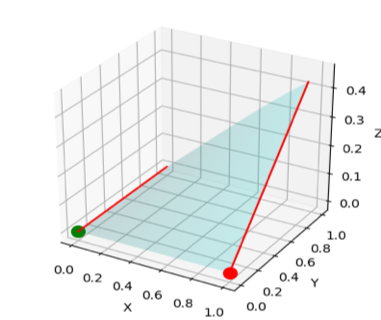
\includegraphics[width=0.4\linewidth]{simulation/incremental}
	\caption{Tool path between two successive blade locations.}\label{fig:incremental}
\end{figure}

% At-every-iteration of the simulation, a geometric master model locates the surgical tools, resolves tool-tissue collisions and tissue-tissue collisions, and communicates this information to the finite element model.

Incremental updating of the BVH geometry model and FE physics models are essential for real-time cutting procedure simulation. The key to incremental cutting is to reuse as much state information as possible from the previous steps and express a new cut state as a minimal and low rank update of the previous one. The figure below shows an example of single tetrahedral being cut incrementally, where the added sub-tetrahedra generate the necessary updates that are passed to the BVH and FE models. These updates involve information about deleted edges and faces as well as newly added ones. These updates are obviously much smaller in size than the model size, and can therefore be quickly incorporated in the BVH and FE models, as well as the rendering and UI modules of the system. The efficient collection and communication of these changes (also known as topology deltas) are key to the successful integration of the different modules. This was implemented within the cutting system to allow efficient fine-grained communication between the different modules. The system keeps track of all new tetrahedra along with the new and deleted edges and faces per cutting step and communicates the strict necessary information to the other modules.


% We have finished the implementation and testing of the incremental solution strategy which relies on a state machine to change elements from one cut state to another and generate the necessary updates.

\begin{figure}
  \centering%
  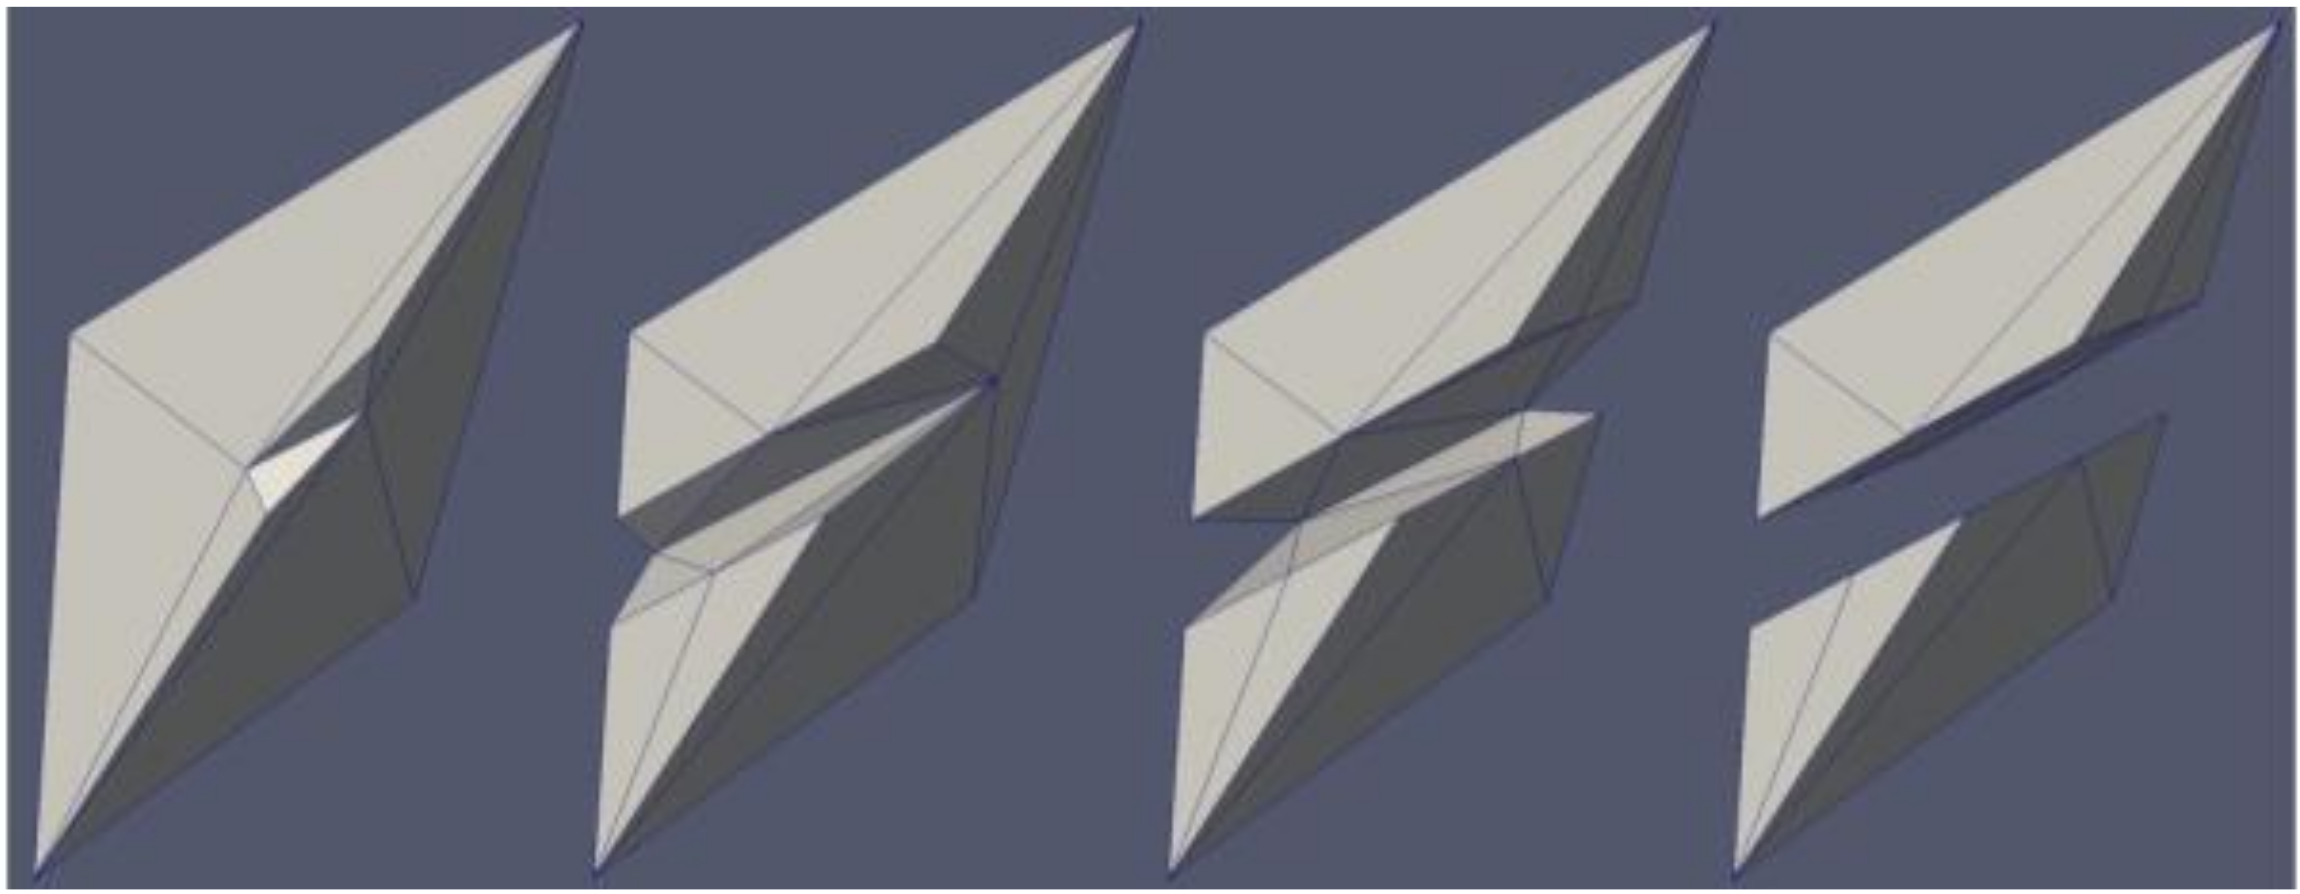
\includegraphics[width=0.7\linewidth]{simulation/cut_progression}
  \caption{Progressive cut of tetrahedral element.}\label{fig:discontinuous_tetrahedra_solver}
\end{figure}

Specifically, the fast incremental solver needs a fine-grained communication with a \acr{bvh}, a powerful data structure for tracking geometric objects and accelerating geometric operations such as triangle-segment intersections ubiquitous in the cutting module. An \acr{api} was designed and implemented to allow the cutting module to communicate information to the \acr{bvh}. In particular, the \acr{bvh} \acr{api} allows the cutting module to determine which edges and faces of the mesh have been cut by a particular sweep of a cutting tool, as well as the geometries of these intersections, in logarithmic complexity. The \acr{bvh} module also requires information about all changes in the mesh to be able to update and restructure the hierarchy so it is synchronized with the base mesh to continue supporting intersection queries. 


The FE model has to also update the solution, including the displacements of the model and the stresses in it, based on the new geometry (cut location) and any contact constraints between tools and tissue. Resolving the finite element system from scratch with every tool movement would preclude real-time operation. Therefore, incremental solution strategies that exploit the nature of the changes to generate the updated displacements and stresses are needed. These changes in the model and contact constraints are formulated as low rank updates of the finite element stiffness matrix and its factorization. As with BVH, the key to fast incremental solution is the efficient two-way fine-grained communication between the finite element system and the collision detection and intersection computation system which incorporates bounding volume hierarchy of the geometric representation. The geometric computation system returns intersection information that is used to build incrementally a set of constraints and/or a set of cuts in the volumetric mesh, as well as \enquote{topology deltas} indicating which elements have been removed and which new elements were added. This incremental communication allows fast updates to the factorization of the finite element stiffness system matrix
 and the resulting solution. 

Furthermore, cutting the mesh produces modifications and this information must be communicated with the other modules of the system. 
For example, the \acr{ui} requires the new surface triangles that are created as the mesh opens up after the cut in order to render the new shape of the mesh. 

The result is a complete system controllable through a \acr{ui} that can cut open a volumetric mesh in real time. Cuts can have sharp curvatures---sharper than those that are resolved by the geometric mesh; cuts are incremental: they can completely separate the \acr{3d} mesh or only partially open it; cuts can also intersect each other. We believe these capabilities surpass the state of the art in this area and our early presentations of the system at international conferences have been very well received, with leading groups from around the world requesting access to the system. Below is a screenshot from the running system. Sample animation videos are available at \url{https://www.dropbox.com/s/ly53lbgmy1m2aw2/animm-4cuts.avi} and \url{https://www.dropbox.com/s/rjmw8avzb0dkwpm/animm-liver.avi}.

\begin{figure}
	\centering%
	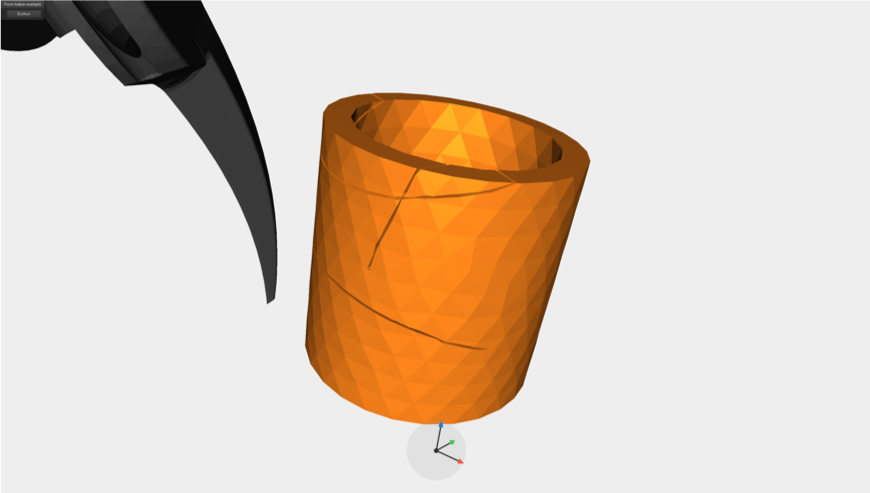
\includegraphics[width=\linewidth,frame]{simulation/endo_cut}
	\caption{Multiple cuts of a cylindrical model.}
	\label{fig:endo_cut}
\end{figure}

\autoref{fig:contact} shows a typical cutting scenario that involves a deformation of the soft tissue by a tool followed by a snipping motion in the case of scissors (the transparent triangular surface shows the snipping motion of the blades of the scissors).
\autoref{} shows various geometrically complex cut paths of a solid sphere discretized by tetrahedral elements to demonstrate the general flexibility and reliability of the progressive cutting procedures.
\begin{figure}
  \centering%
  \setlength{\fboxsep}{0pt}%
  \setlength{\fboxrule}{0.1pt}%
  \fbox{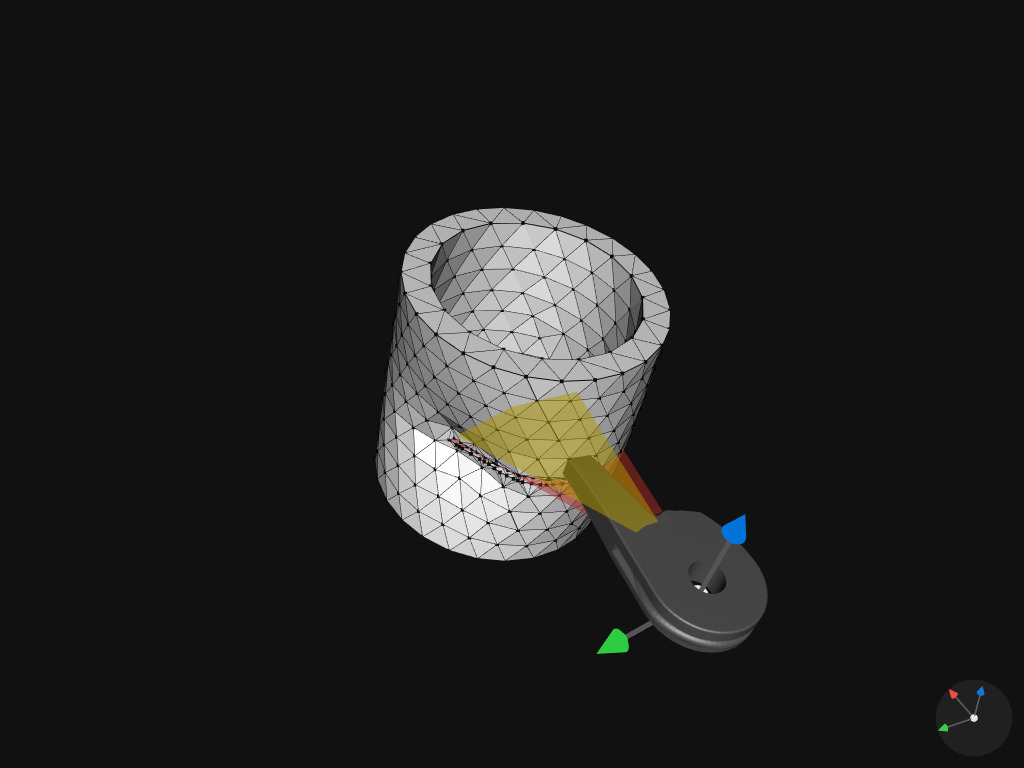
\includegraphics[width=0.5\linewidth]{simulation/snip3}}
  \caption{Deforming and snipping a tube}\label{fig:contact}
\end{figure}

\begin{figure}
  \centering%
	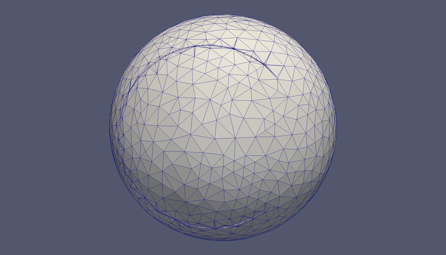
\includegraphics[width=0.4\linewidth]{simulation/sphere_1}\hfill%
	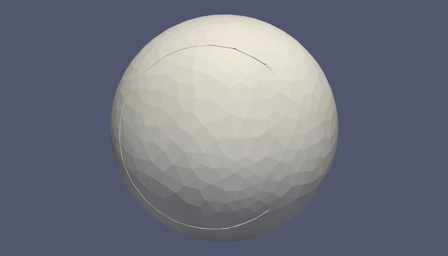
\includegraphics[width=0.4\linewidth]{simulation/sphere_2}\\[1.5ex]
	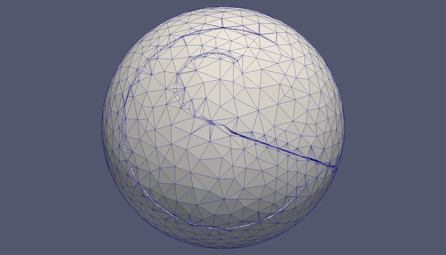
\includegraphics[width=0.4\linewidth]{simulation/sphere_3}\hfill%
	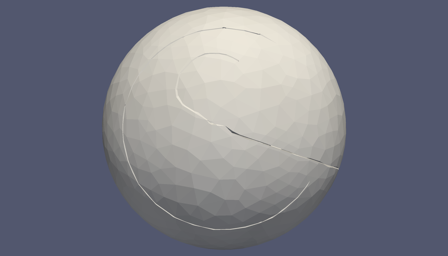
\includegraphics[width=0.4\linewidth]{simulation/sphere_4}\\[1.5ex]
	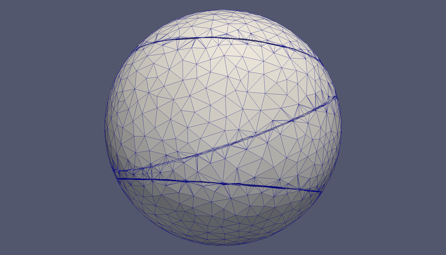
\includegraphics[width=0.4\linewidth]{simulation/sphere_5}\hfill%
	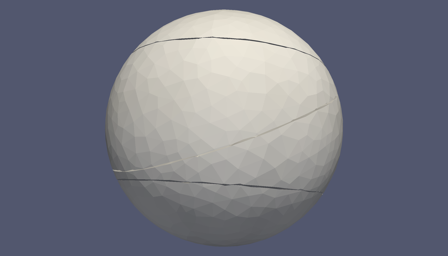
\includegraphics[width=0.4\linewidth]{simulation/sphere_6}\\
	\caption{Examples of geometrically complex cuts of a spherical mesh.}\label{fig:sphere}
\end{figure}


% Timings of the various steps in the process have been performed. The results of the timings identified one bottleneck that could prevent real-time interaction as the constrains set size increases. Optimizations we performed as a result to remove inactive constraints prior to entering the solution loop. This resulted in a much more responsive system with a stable interaction time for the kinds of meshes needed when cutting urethra and models of similar complexity.



% ======================================================================

\subsection{Non-linear Solver}\label{ssec:nonlinear_solver}
% The nonlinear solver is necessary when large deformations take place. The solution strategy in this case involves an iterative Newton-like scheme that builds on the linear solve. The challenge for the non-linear solution is to control both the number of iterations and the cost of solving the modified linear problem at every iteration. We have started the development of a strategy that performs an approximate solution for the modified problem at every iteration, based on a hierarchical matrix representation of the stiffness matrix which produce algebraic approximations of off-diagonal matrix blocks and can substantially speed up the solution process.

In simulations of cutting procedures, large deformations generally take place necessitating a nonlinear solution strategy that handles the large kinematics of these deformations. \autoref{fig:tube} shows an example of such deformation where a tube under tension is snipped incrementally. Modifications to the underlying tetrahedral model are generated automatically as the tube is sniped around a cross section by a scissor tool (not shown), and the resulting large nonlinear tube deformations are shown.

\begin{figure}
  \centering%
	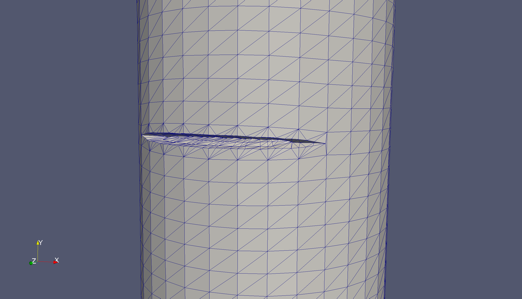
\includegraphics[width=0.22\linewidth]{simulation/tube_1}\hfill%
	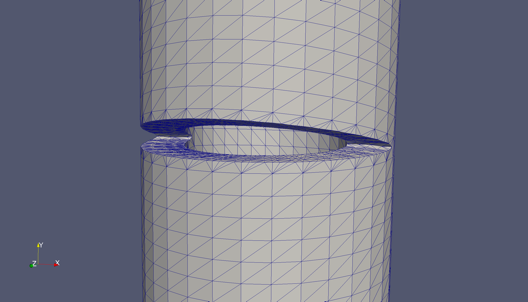
\includegraphics[width=0.22\linewidth]{simulation/tube_2}\hfill%
	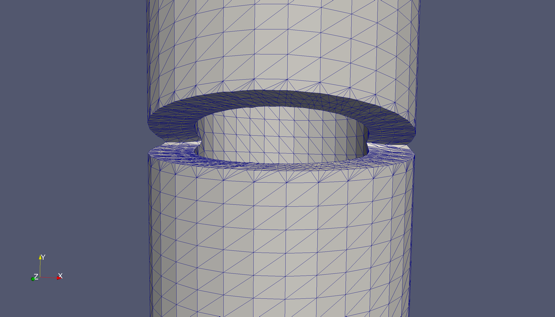
\includegraphics[width=0.22\linewidth]{simulation/tube_3}\hfill%
	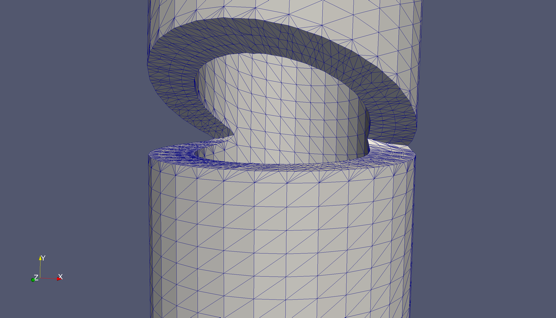
\includegraphics[width=0.22\linewidth]{simulation/tube_4}\\

  \centering%
	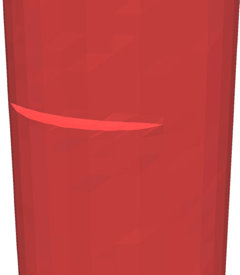
\includegraphics[width=0.2\linewidth]{simulation/tube_5}\hfill%
	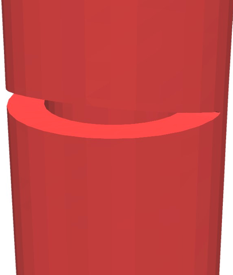
\includegraphics[width=0.2\linewidth]{simulation/tube_6}\hfill%
	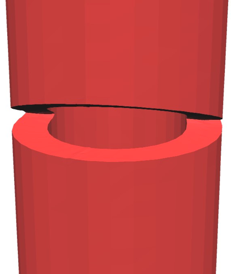
\includegraphics[width=0.2\linewidth]{simulation/tube_7}\hfill%
	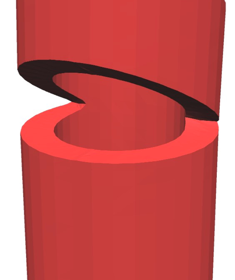
\includegraphics[width=0.2\linewidth]{simulation/tube_8}\\
	\caption{Progressive cut of a tubular shape (mesh, top; and rendered shape, bottom).}\label{fig:tube}
\end{figure}

We handle the nonlinearities using a local-global strategy, and assume the strain energy of the system
comes from the edges of the mesh. The local-global strategy reformulates the potential energy 
of the system as a minimization problem and introduces auxiliary variables
corresponding to the rest-length of the elements. This new problem is linear in the 
positions of the nodes, and non-linear in the newly introduced variable. 
By employing block coordinate descent, we can iteratively solve for the spring 
directions and node positions separately, allowing us to split each iteration 
into a simple non-linear local problem with a solution in closed form, and a
linear problem involving the global stiffness matrix. Furthermore, the linear problem is independent of the system
state, allowing us to benefit from pre-factoring or pre-inverting the system matrix.
Although this method converges slower than Newton's method in terms of the
number of iterations, it is more work-efficient and the low 
computational cost of an iteration makes up for the slow convergence.

Consider a system with $m$ nodes and $s$ elements. Let $\mathbf{K}$ be the stiffness 
matrix of the system, and let $\mathbf{J}$ be the matrix consisting 
the stiffness weighted incidence vectors of the springs in its columns. 
The potential energy of the system can be expressed in the following minimization 
problem:
\begin{equation}
  E(x) = \min_{\|\mathbf{d}_i\| = r_i} \ 
  \frac{1}{2}\mathbf{x}^\intercal\mathbf{Kx} -
  \mathbf{x}^\intercal\mathbf{Jd}
\end{equation}
where $\mathbf{x}$ represents the node positions, $\mathbf{d}$ the spring 
directions, and $r_i$ the rest length of the \textit{ith} spring. To model
bending resistance for surface elements, a quadratic bending 
energy model presented in \cite{Bergou06} is used. 

$\mathbf{K}$ can be expressed as the sum of rank-one matrices: 
\begin{equation}
  \mathbf{K} = \sum_{i = 1}^s k_i\mathbf{A}_i\mathbf{A}_i^\intercal
\end{equation}
where $\mathbf{A}_i \in R^{m}$ are the spring incidence vectors and 
We  make use of this fact to directly update the inverse of $\mathbf{K}$ (or
equivalently, its Cholesky factors), allowing for fast interactive cutting.
%------------------------------------------------

% In this section, we outline the parallel implementation of the implicit integrator,
% introduce the cutting algorithm, and present a method for augmenting the system
% to introduce physically-based external interaction.

\subsubsection{Parallel Integrator}
The solution framework is described next, and is implemented both for multicore CPUs as well as GPUs.  
Each iteration of the integrator for this framework consists of the following steps:
\begin{enumerate}
  \item Compute the element directions $\mathbf{d}$.
  \item Compute $\mathbf{Jd}$.
  \item Solve $\mathbf{Kx} = \mathbf{Jd}$.
  \begin{enumerate}
    \item Sparse Cholesky factorization
    \begin{enumerate}
      \item Permute the right-hand side $\mathbf{P^\intercal Jd}$.
      \item Solve the equation $\mathbf{(P^\intercal KP)(P^\intercal x)} = \mathbf{P^\intercal Jd}$.
      \item Unpermute the solution $\mathbf{PP^\intercal x} = \mathbf{x}$.
    \end{enumerate}
    % \item Dense matrix inverse
    % \begin{enumerate}
    %   \item Compute $\mathbf{x} = \mathbf{K^{-1}Jd}$.
    % \end{enumerate}
  \end{enumerate}
 
  \item Repeat from step 1.
\end{enumerate}
where $\mathbf{P}$ is the approximate minimum degree permutation of the
Cholesky factorization of $\mathbf{K}$. 

Steps 1 and 2 are fairly straight forward to parallelize. In step 1, we
launch a kernel where each thread computes the direction of a single spring.
This involves normalizing each spring direction and multiplying by the corresponding
rest-length. Step 2 is implemented as a level 3 sparse BLAS operation.

Step 3 uses a pre-computed Cholesky factorization of
$\mathbf{K}$ to perform a sparse triangular solve. However, due to the inherently
serial nature of triangular solvers, this will have to be preceded with an 
analysis phase to extract as much parallelism as possible \cite{Mayer09}.
Furthermore, the permutation
required at every iteration is a potential performance bottleneck, since it is 
highly memory bound. However, this can easily be avoided by computing all 
iterations in the permuted space, thus only permuting at the very first and 
very last iterations.

Another approach for the linear solution is to pre-compute $\mathbf{K^{-1}}$ and solve the system
using dense matrix multiplication. Although this is expected to perform
extremely well on GPUs, it might not be feasible to store the inverse
for very large matrices and will not scale well. 

\subsubsection{Effects of cuts on the solver}
Cuts in the mesh are incorporated into the model by deleting and adding elements. Suppose we delete
$n$ elements, where each element has a rank-one contribution to the system matrix. 
This cut corresponds to the following low-rank update:
\begin{equation}
  \mathbf{K}:=
  \mathbf{K} - \mathbf{U}\mathbf{U^\intercal}
\end{equation}
where $\mathbf{U} \in R^{m \times n}$ encapsulates the contributions
of all the deleted springs. 

Thus, we can directly update the Cholesky factors or the inverse of the
system matrix. For example, using the dense solver approach we can update
$\mathbf{K^{-1}}$ using the Sherman-Morrison identity:
\begin{equation}
  \mathbf{K}^{-1} :=
  \mathbf{K}^{-1} +
  \mathbf{K}^{-1}\mathbf{U}(\mathbf{I} - \mathbf{U^\intercal K}^{-1}\mathbf{U})^{-1}
  \mathbf{U^\intercal K}^{-1}
\end{equation}
% First, we intersect the edges of the mesh with a cutting surface and accumulate
% the intersected edges in a buffer. These edges are then deleted from the mesh.
In the case of the GPU implementation, the ``topological deltas'' are accumulated in 
an edge buffer and transfered to the GPU and a kernel is launched to construct
the matrix $\mathbf{U}$. The Sherman-Morrison identity involves dense matrix
multiplication and inversion, which have fast parallel implementations. 


\subsubsection{Interaction}
A slight modification of the basic solution strategy is needed to 
allow for user interaction using dynamic constraints.
We can constrain any point on the mesh surface using the method of
Lagrange multipliers. First, the constrained point $\mathbf{p_i}$ is expressed as a linear 
combination of one, two or three vertices:
\begin{equation}
\label{eq:lin_comb}
\mathbf{p_i} =
\alpha_{i_1} \mathbf{x_{i_1}} +
\alpha_{i_2} \mathbf{x_{i_2}} +
\alpha_{i_3} \mathbf{x_{i_3}} =
\mathbf{C_{i,:} x},
\end{equation}
where \autoref{eq:lin_comb} can be thought of as a constraint of the original minimization 
problem. Next, we augment the orignal linear system with these constraints via the 
following reformulation:
\begin{equation}
    \begin{bmatrix}
        \mathbf{K} & \mathbf{C}^\intercal \\
        \mathbf{C} & \mathbf{0}
    \end{bmatrix}
    \begin{bmatrix}
        \mathbf{x} \\
        \boldsymbol{\lambda}
    \end{bmatrix}
    =
    \begin{bmatrix}
        \mathbf{Jd} \\
        \mathbf{p}
    \end{bmatrix}
\end{equation}
where $\boldsymbol{\lambda}$ corresponds to the Lagrange multipliers of the 
constrained problem, and $\mathbf{p}$ to the positions of the constrained points.
To allowing for dynamic resizing of $\mathbf{C}$ without having to continuously
update the linear system, we reduce the system to the following form:
\begin{equation}
    \begin{bmatrix}
        \mathbf{K} & \mathbf{C}^\intercal \\
        \mathbf{0} & -\mathbf{CK^{-1}C^\intercal}
    \end{bmatrix}
    \begin{bmatrix}
        \mathbf{x} \\
        \boldsymbol{\lambda}
    \end{bmatrix}
    =
    \begin{bmatrix}
        \mathbf{Jd} \\
        \mathbf{p} - \mathbf{CK^{-1}Jd}
    \end{bmatrix}
\end{equation}
where $\mathbf{C}$ can now be updated separately from $\mathbf{K}$,
at the cost of having to solve for $\boldsymbol{\lambda}$ in a separate step.
% \begin{figure}[ht]
%   \centering
%   \includegraphics[width=0.25\textwidth]{images/shirt_push_no_back.png}
%   \caption{
%     Dynamic constraints allow for physically based interaction without
%     the cost of continuously updating the entire linear system.
%   }
%   \label{fig:shirt-push}
% \end{figure}

%------------------------------------------------


\subsubsection{Results}
\begin{figure}
  \centering
  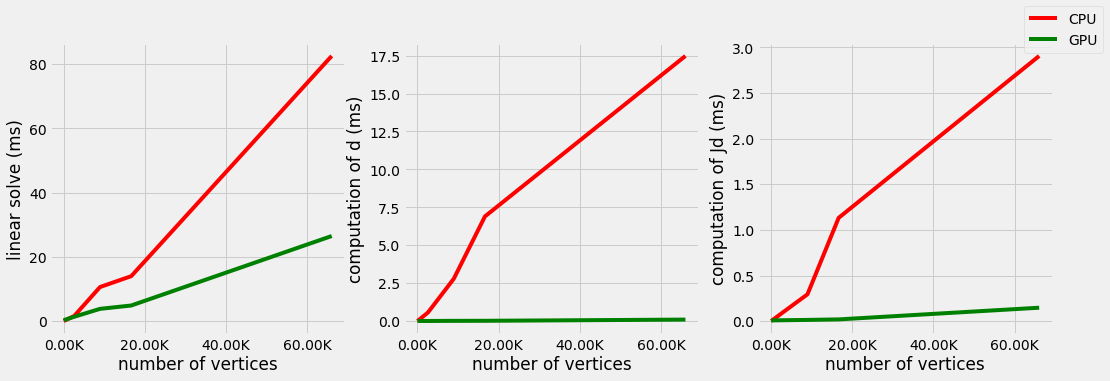
\includegraphics[width=1.0\textwidth]{simulation/performance_plots.png}
  \caption{
    Performance of different stages of a single iteration of the 
    sparse serial and parallel implementations. From left to right:
    linear solve, computation of $\mathbf{d}$, computation of $\mathbf{Jd}$.
  }
  \label{fig:performance-iteration}
\end{figure}

Figure \ref{fig:performance-iteration} illustrates the performance of this framework.
Each graph shows the execution time of the serial and parallel implementations of
an iteration of the sparse integrator on an increasing
number of vertices. This performance allows us to execute a large number of iterations in real-time. 
Table \ref{table:dense} shows how the dense integrator significantly outperforms 
both the serial and parallel sparse implementations for a relatively small mesh. However, 
the polynomial complexity of the dense representation will not scale. 

\begin{table}[ht]
\caption{Performance of the different solvers on small meshes.}
\centering
\begin{tabular}{lrrr}
\toprule
\multicolumn{3}{r}{Execution Time (ms)} \\
\cmidrule(r){2-4}
\textit{m} & Sparse(CPU) & Sparse (GPU) & Dense (GPU) \\
\midrule
% $9$ & $0.002$& $0.320512$ & $0.007328$ \\
$2590$ & $1.575$ & $1.33437$ & $0.202816$ \\
\bottomrule
\end{tabular}
\label{table:dense}
\end{table}


% We have started the development of a refinement of our non-linear solver that has the potential to produce two key advantages:
% \begin{enumerate*}[(1)]
%   \item it allows a straightforward mechanism for trading real-time solution speed and efficiency with solution accuracy.  We have found that when complex maneuvers are performed on a deformable mesh, a reasonably sizeable subset of teteraheda, faces, and edges may be affected. Resolving all these changes to high-accuracy in real time is not possible. Therefore, an elegant solution is to maintain real-time rates of interaction and display, but allow slightly lower fidelity in the rendered deformations.  This lower-fidelity rendering is only transient however. As soon as the complex maneuver that induces large topological changes slows down, the solver \enquote{catches up} and is able to resolve the deformation to the desired higher accuracy;
%   \item it allows a pre-computed factorization of the system matrix to be reused even when a large portion of the model undergoes large rotations requiring non-linear kinematics to be recomputed for a large set of elements. The system stiffness matrix factorization is updated, very efficiently via low rank updates, only when topological changes are introduced by cutting or suturing.  The refined non-linear solution algorithm is effectively an alternating minimization procedure that alternates on updating nodal positions and element deformations/orientations. The element deformations updates are local in nature, providing a substantial algorithmic benefit. The description of this algorithm and its performance in the context of our overall cutting system will be submitted for publication later this summer.
% \end{enumerate*}
%
% We have wrapped up and tested the developments of the non-linear solver algorithm. Our algorithm is particularly designed for real-time interaction as it allows a pre-computed factorization of the system matrix to be reused even when a large portion of the model undergoes large rotations requiring non-linear kinematics to be recomputed for a large set of elements. The alternating minimization procedure used in the solver alternates on updating nodal positions and element deformations/orientations. The element deformations updates are local in nature, providing a substantial algorithmic benefit particularly on \acr{gpu}'s. A \acr{gpu} kernel to compute the local updates in parallel has been developed to be used in tandem with the stiffness matrix factorization, updated as cuts are introduced.
%
% Fine-tuning and calibrations of the parameters of the non-linear solver were also performed.  The  solver iterates on two types of nonlinearities:
% \begin{enumerate*}[(1)]
% \item the \enquote{outer} non-linearity which involves the active set of constrains; the solution algorithm must iterate until this active set is stable; and
% \item non-linearity of the deformations for a given set of active constraints; this is the inner loop of the iteration and does not need to be solved to final accuracy until a stable active constraint set has been identified.
% \end{enumerate*}




% ======================================================================
 
\subsection{GPU Acceleration}\label{ssec:gpu_acceleration}

The solution of the underlying large system of algebraic equations is the main time-consuming portion of a finite element simulation, and it is therefore critical to accelerate this step using \acr{gpu} parallel hardware. The sparse factorization described in the previous section suffers from two difficulties on parallel GPU hardware. Its memory footprint and the number of FLOPS it requires scale superlineary with problem size because of fill-in, and the triangular sparse solves introduce an inherent serialization in the solution which prevent efficient parallel execution on manycore processors. As a scalable alternative strategy on GPUs, we generate the inverse stiffness matrix in a hierarchical matrix representation format requiring only linear memory footprint.  This reduces the solution problem to multiplying this matrix by a force vector, which can be parallelized very effectively. 

Hierarchical matrices are space and time efficient representations of dense matrices that exploit the low rank structure of matrix blocks at different levels of granularity. The hierarchically low rank block partitioning produces representations that can be stored and operated on in near-linear complexity instead of the usual polynomial complexity of dense matrices. In the context of real-time simulation, this near-linear growth is key for the simulation of large realistic models. \autoref{fig:gpu_matrix} below show how a hierarchical matrix is partitioned: some blocks (shown in red) are stored as regular dense matrices, while others of differing sizes are stored as low rank blocks.


\begin{figure}
  \centering%
	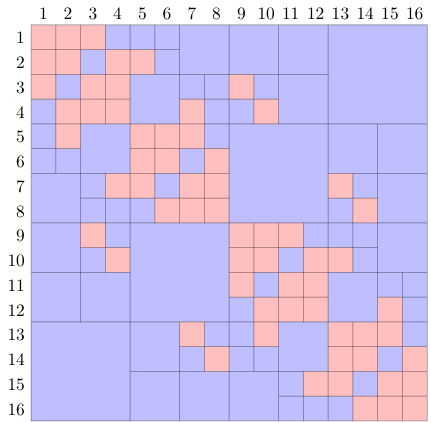
\includegraphics[width=0.4\linewidth]{simulation/GPU_block}\vspace{2ex}
	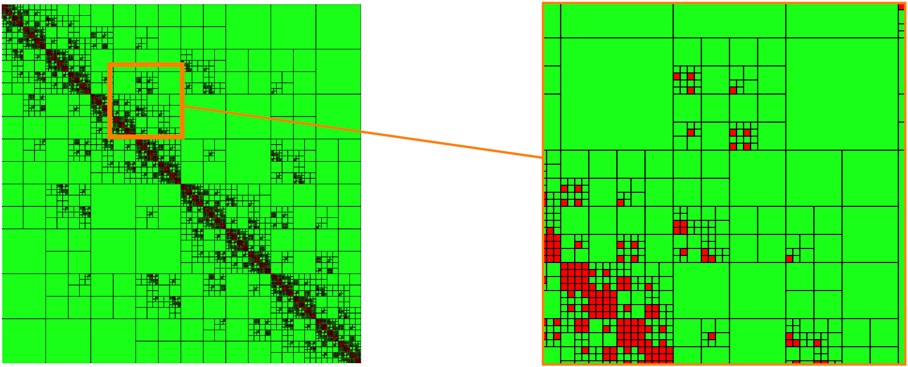
\includegraphics[width=0.9\linewidth]{simulation/GPU_zoom}\\
	\caption{Hierarchical matrix representation: dense blocks are shown in red; the rest of the matrix consists of low rank blocks at different level of granularities.}\label{fig:gpu_matrix}
\end{figure}


The challenges in developing efficient data-parallel \acr{gpu} algorithms come primarily from the irregular tree data structures that underlie the hierarchical representations, and the key to performance is to recast the computations on flattened trees in ways that allow batched linear algebra operations to be performed. We developed new \acr{gpu} algorithms in both \acr{sp} and \acr{dp}. Streams are used to overlap various stages of the computation and hide latencies. Sample performance results are shown in \autoref{fig:gpu_performance}. Our hierarchical matrix-vector multiplication 
(\acr{hmvm}) \acr{gpu}-accelerated routines involved in the finite element solution can generate solutions in less than \SI{5}{\milli\second} on a problem with 260 K degrees of freedom, and can achieve over \SI{550}{\giga\byte/\second} on the P100 Pascal \acr{gpu}. These results show that the absolute performance of these operations can very effectively leverage the power of \acr{gpu}'s and, perhaps more importantly, that the optimal linear and log-linear growth of these algorithms allow the scaling of our cutting and suturing models beyond what current state of the art systems can do.  

\begin{figure}
  \centering%
	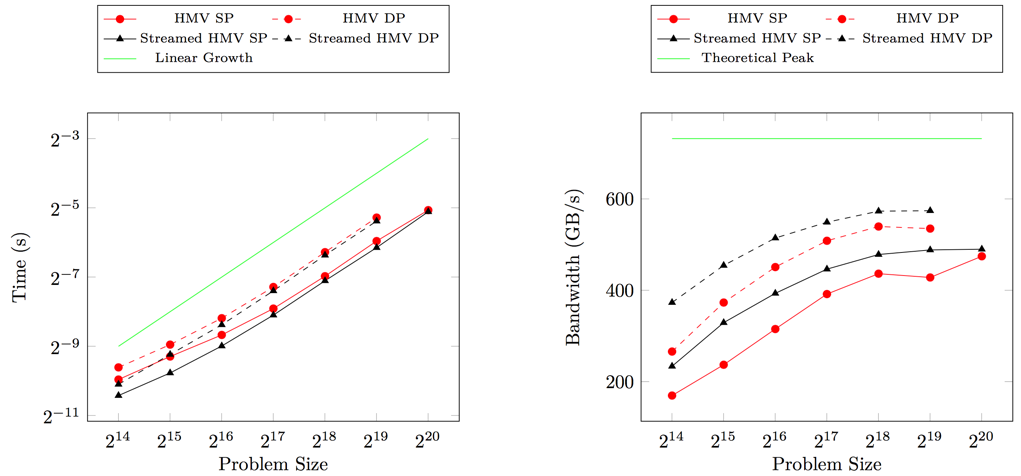
\includegraphics[width=\linewidth]{simulation/GPU_performance}
	\caption{GPU performance of hierarchical matrix-vector multiplication.}\label{fig:gpu_performance}
\end{figure}

We also developed additional \acr{gpu}-accelerated operations including low rank update operations, matrix-matrix multiplication performed by sampling the resulting product using an adaptive randomized approximation (HARA) scheme,  as well as iterative Newton-schulz matrix inversion operations.  These state-of-the-art algorithms push the boundary of what is possible to do in real time on \acr{gpu}'s at the fundamental algorithmic level. Their integration in the simulation system allows us to scale the simulations to higher resolution and higher fidelity models. 

% We have continued the development of \acr{gpu}-accelerated routines for the \acr{hmvm} operations as well as for the low-rank update operations involved in the finite element solution. Our recent publication on this subject was accepted by the prestigious journal ACM Transactions on Mathematical Software,
%
% We have finished the development of algorithms to support the acceleration of the solution computation when running in the presence of \acr{gpu}'s.

% We have also developed routines for the low-rank update operations involved in the finite element solution.
% The system can now build approximate hierarchical matrix representations of inverses of the stiffness matrices and perform low rank update operations on them in their compressed hierarchical form as the cutting operation progresses.

%
% A recent publication documenting various aspects of these developments has been accepted in the flagship SIAM Journal on Scientific Computing. These state-of-the-art algorithms are pushing the boundary of what is possible to do in real time on \acr{gpu}'s, at the fundamental algorithmic level. Their integration in the simulation system is allowing us to scale the simulations to higher resolution and higher fidelity models.

As examples of the high performance of the system, the figure below shows \acr{gpu} timings and scalability results. The left figure shows the time it takes to construct a hierarchical matrix on a representative problem of various sizes on a P100 Nvidia \acr{gpu}, while the middle figure shows the corresponding performance achieved on these problems. Problems of size 16,000, which are already useful for high resolution surgical models, achieve a 100\,GFLOPS/s performance. Larger models achieve even higher performance, and the growth in runtime is only log-linear in problem size. The last plot shows a computation of the inverse of a stiffness matrix using an iterative Newton-Schulz method on a problem of size 4,000. Second order convergence is observed, and the whole computation is \acr{gpu}-resident.

\begin{figure}
  \centering%
  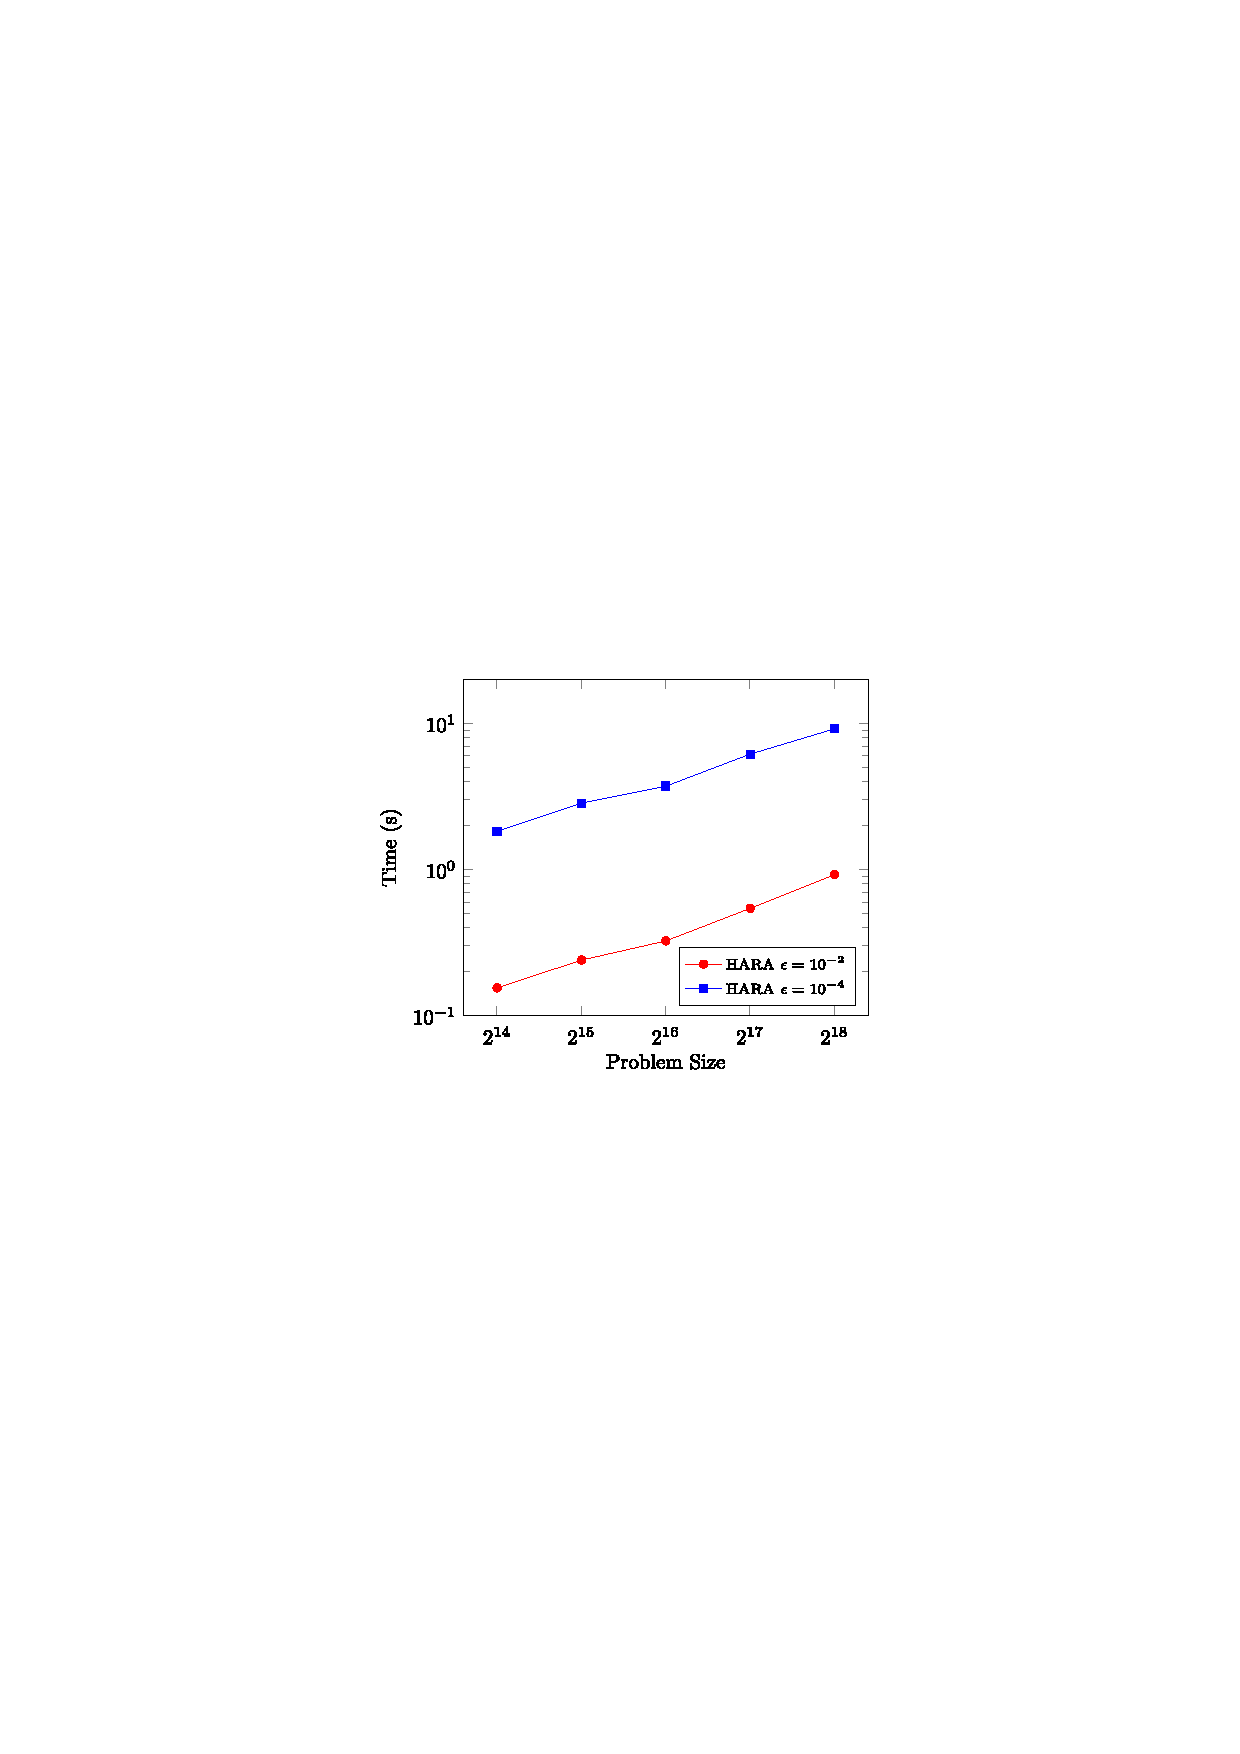
\includegraphics[trim=180 200 160 300,clip,width=0.32\linewidth]{simulation/plot0.pdf}
  \hfill%
  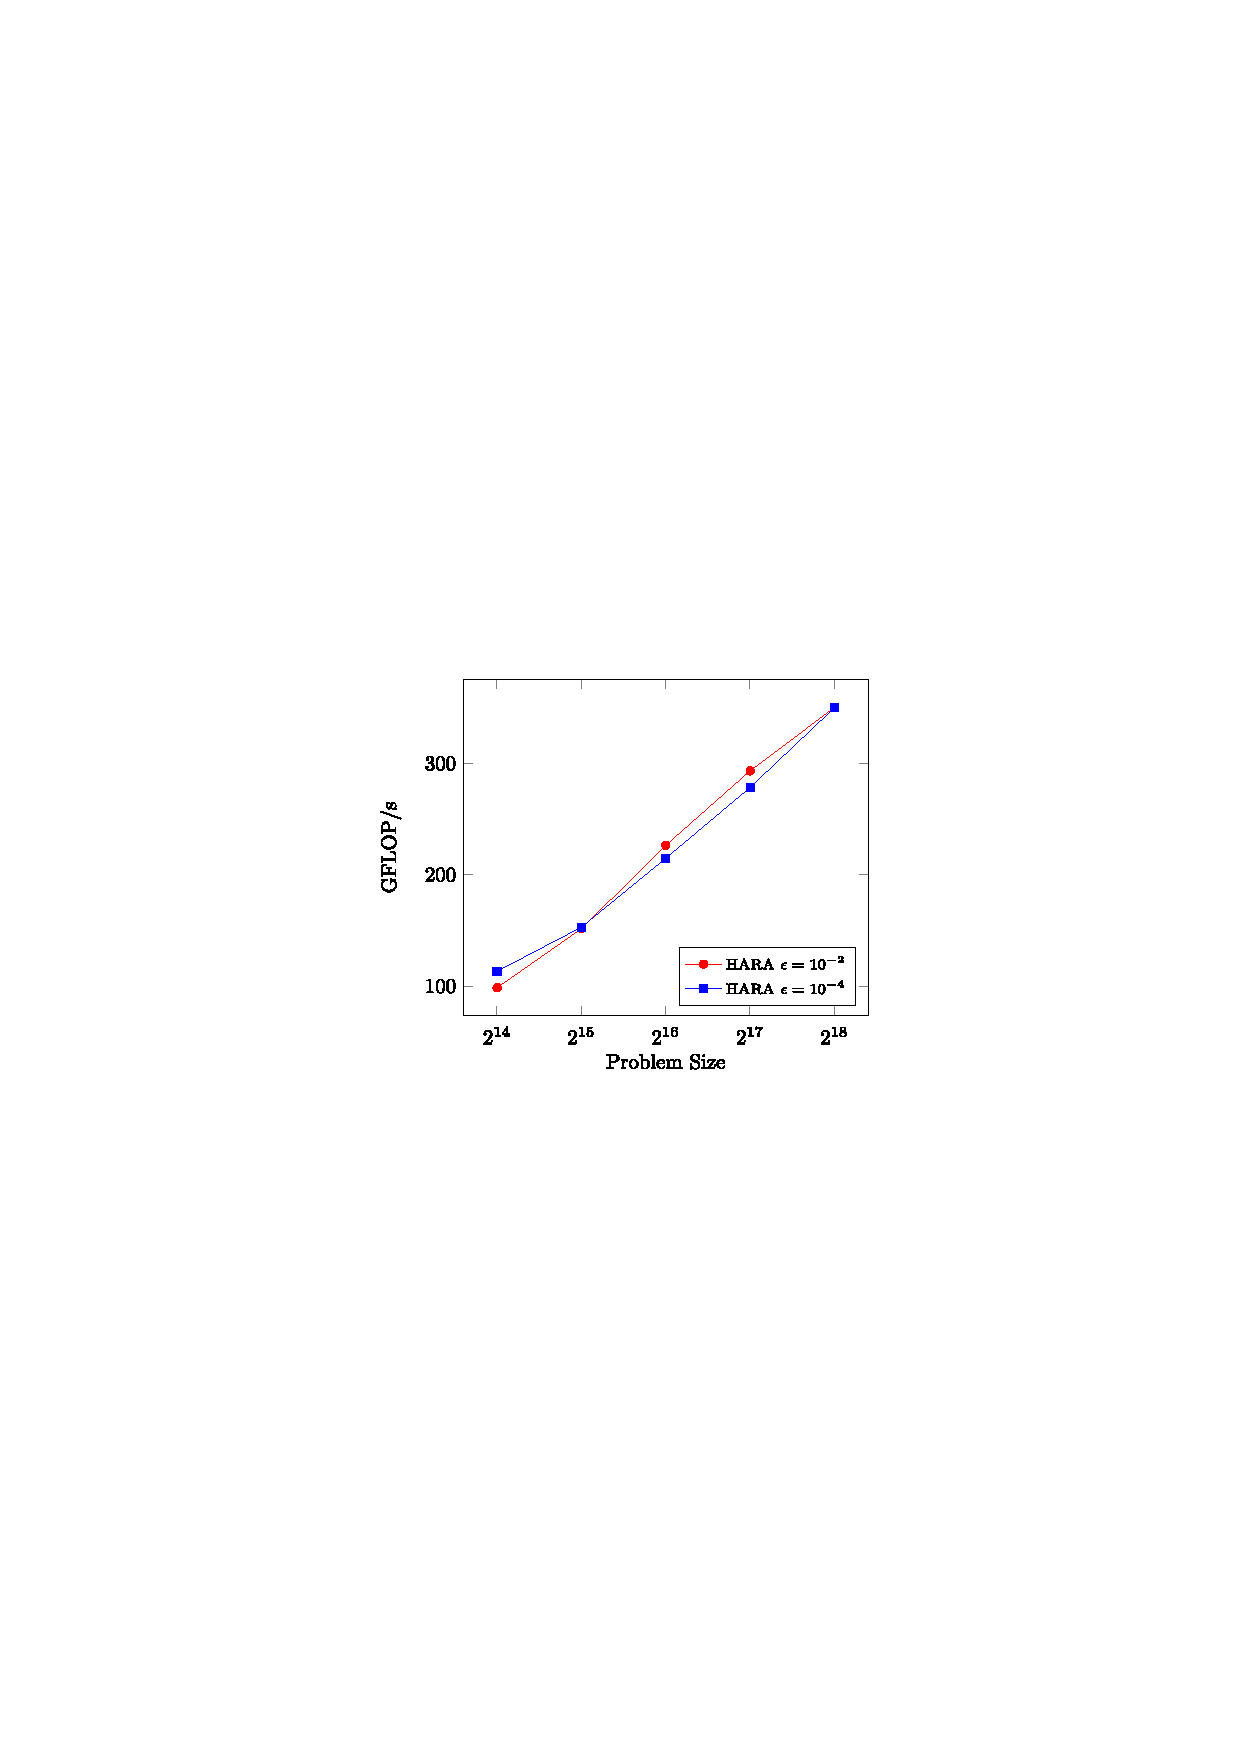
\includegraphics[trim=180 200 160 300,clip,width=0.32\linewidth]{simulation/plot1.pdf}
  \hfill%
  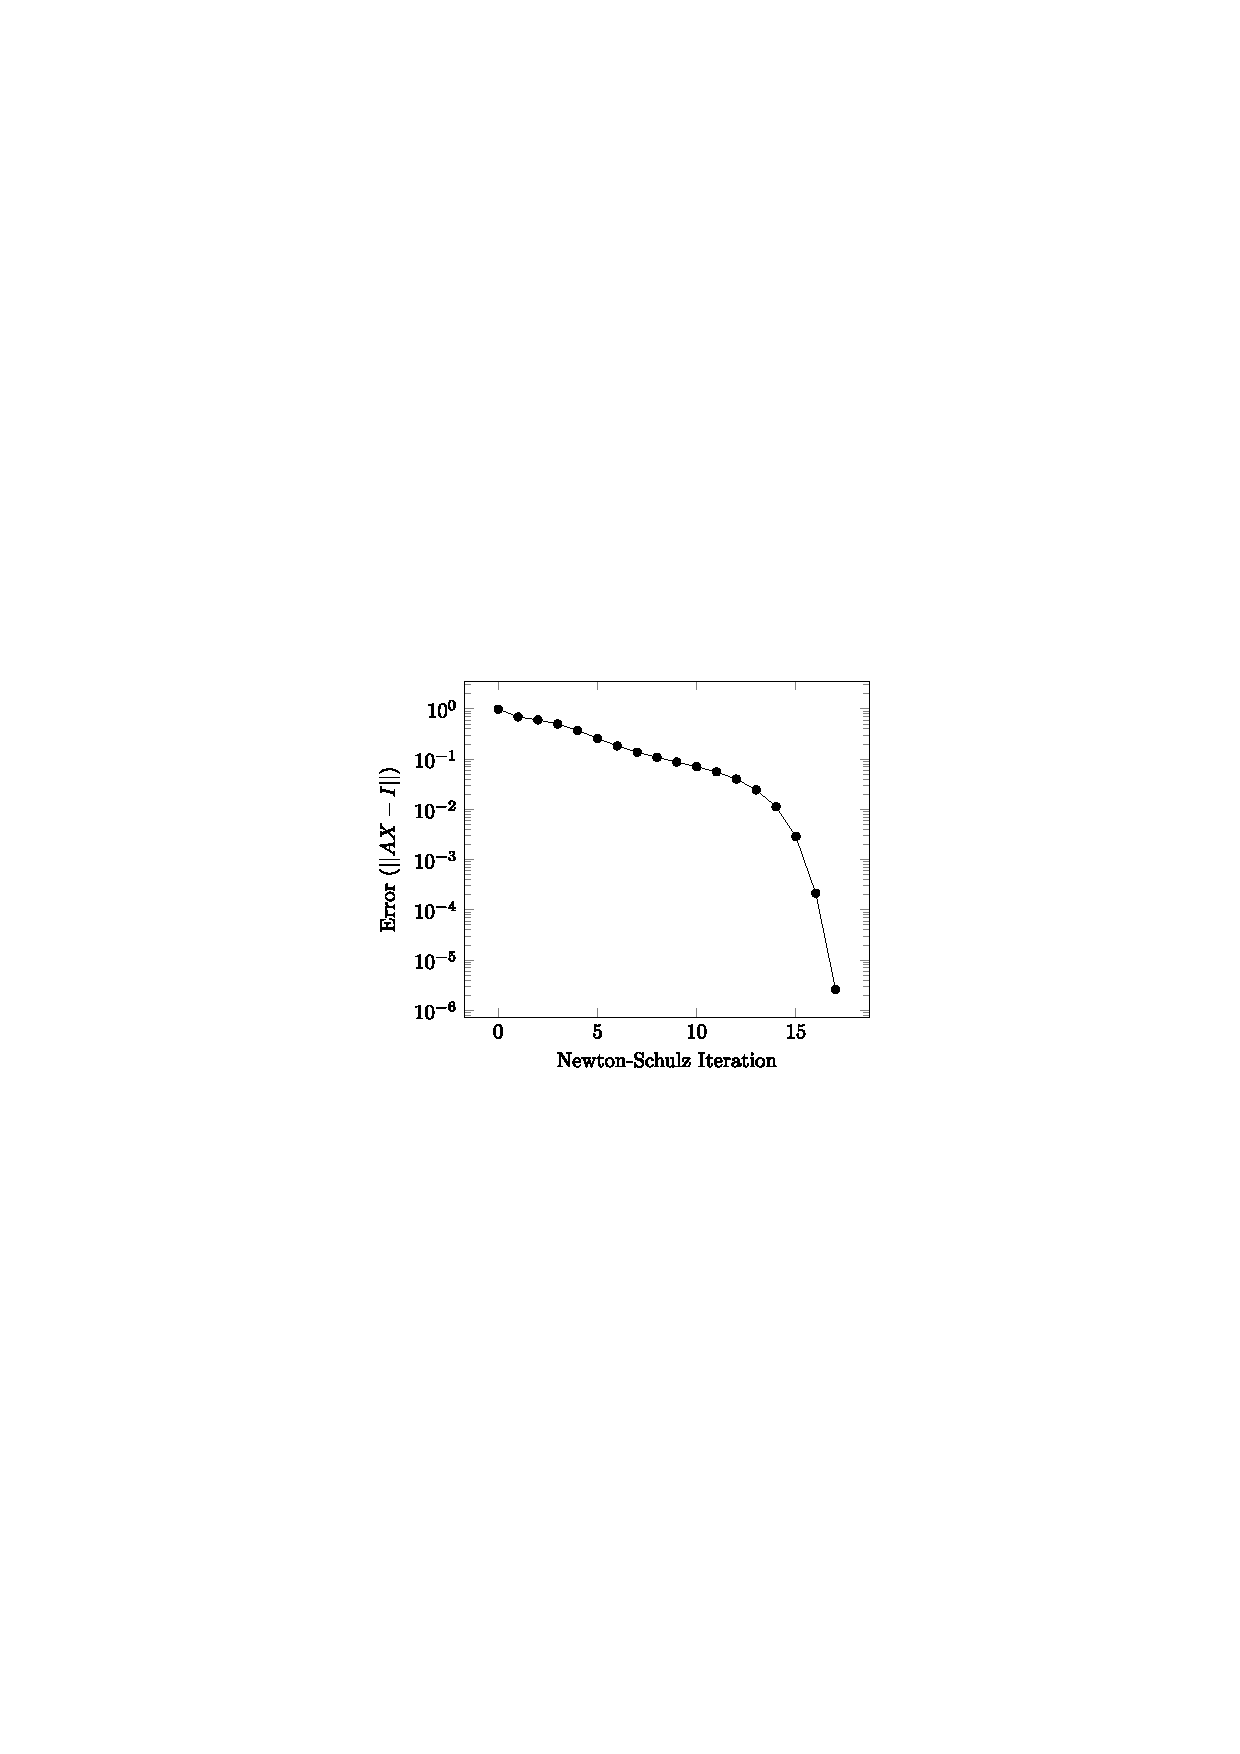
\includegraphics[trim=180 200 160 300,clip,width=0.32\linewidth]{simulation/plot2.pdf}
  \vspace{-15ex}
  \caption{Scalability of GPU-accelerated hierarchical matrix operations.}\label{fig:plots}
\end{figure}

% ==========
% In addition, a hierarchical matrix representation of the system stiffness that replaces the sparse Cholesky factors of the stiffness was also tested and timed. This representation may be used for the solution involving simple deformation constraints and updated, via low-rank matrix updates, to account for cuts introduced. Hierarchical matrix representation is the primary mechanism for getting the solution strategy to run on \acr{gpu}'s, as the sparse matrix factors cannot efficiently take advantage of the many cores of the \acr{gpu}'s.
% =========

\autoref{fig:Htests} compares the effectiveness of the hierarchical matrix representation with that of the sparse Cholesky factorization implemented on GPUs. The time to solution of the hierarchical matrix solution, once the inverse is computed, is shown to be better than that of a forward and backward passes on precomputed Cholesky factors, and the improvement is more significant as the problem size increases. In terms of memory footprint, the hierarchical matrix inverse requires a little more memory than the sparse factors, however the rate of increase of the memory consumption of the hierarchical inverse slows down as the problem size increases and for larger-scale simulations the curves will cross. 

\begin{figure}
  \centering%
  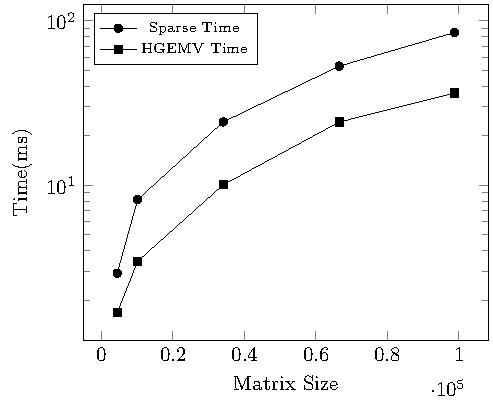
\includegraphics[width=0.4\linewidth]{simulation/sparse_vs_hgemv_time.pdf}	
  \hfill%
  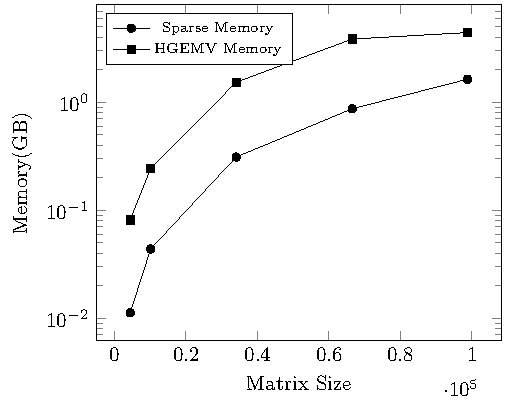
\includegraphics[width=0.4\linewidth]{simulation/sparse_vs_hgemv_memory.pdf}
  \caption{Comparison of hierarchical matrix and sparse factorization solutions on GPUs.}
  \label{fig:Htests}
\end{figure}


\subsection{Faster Time Integration Schemes for Simulation}
\begin{figure}[ht]
  \centering
  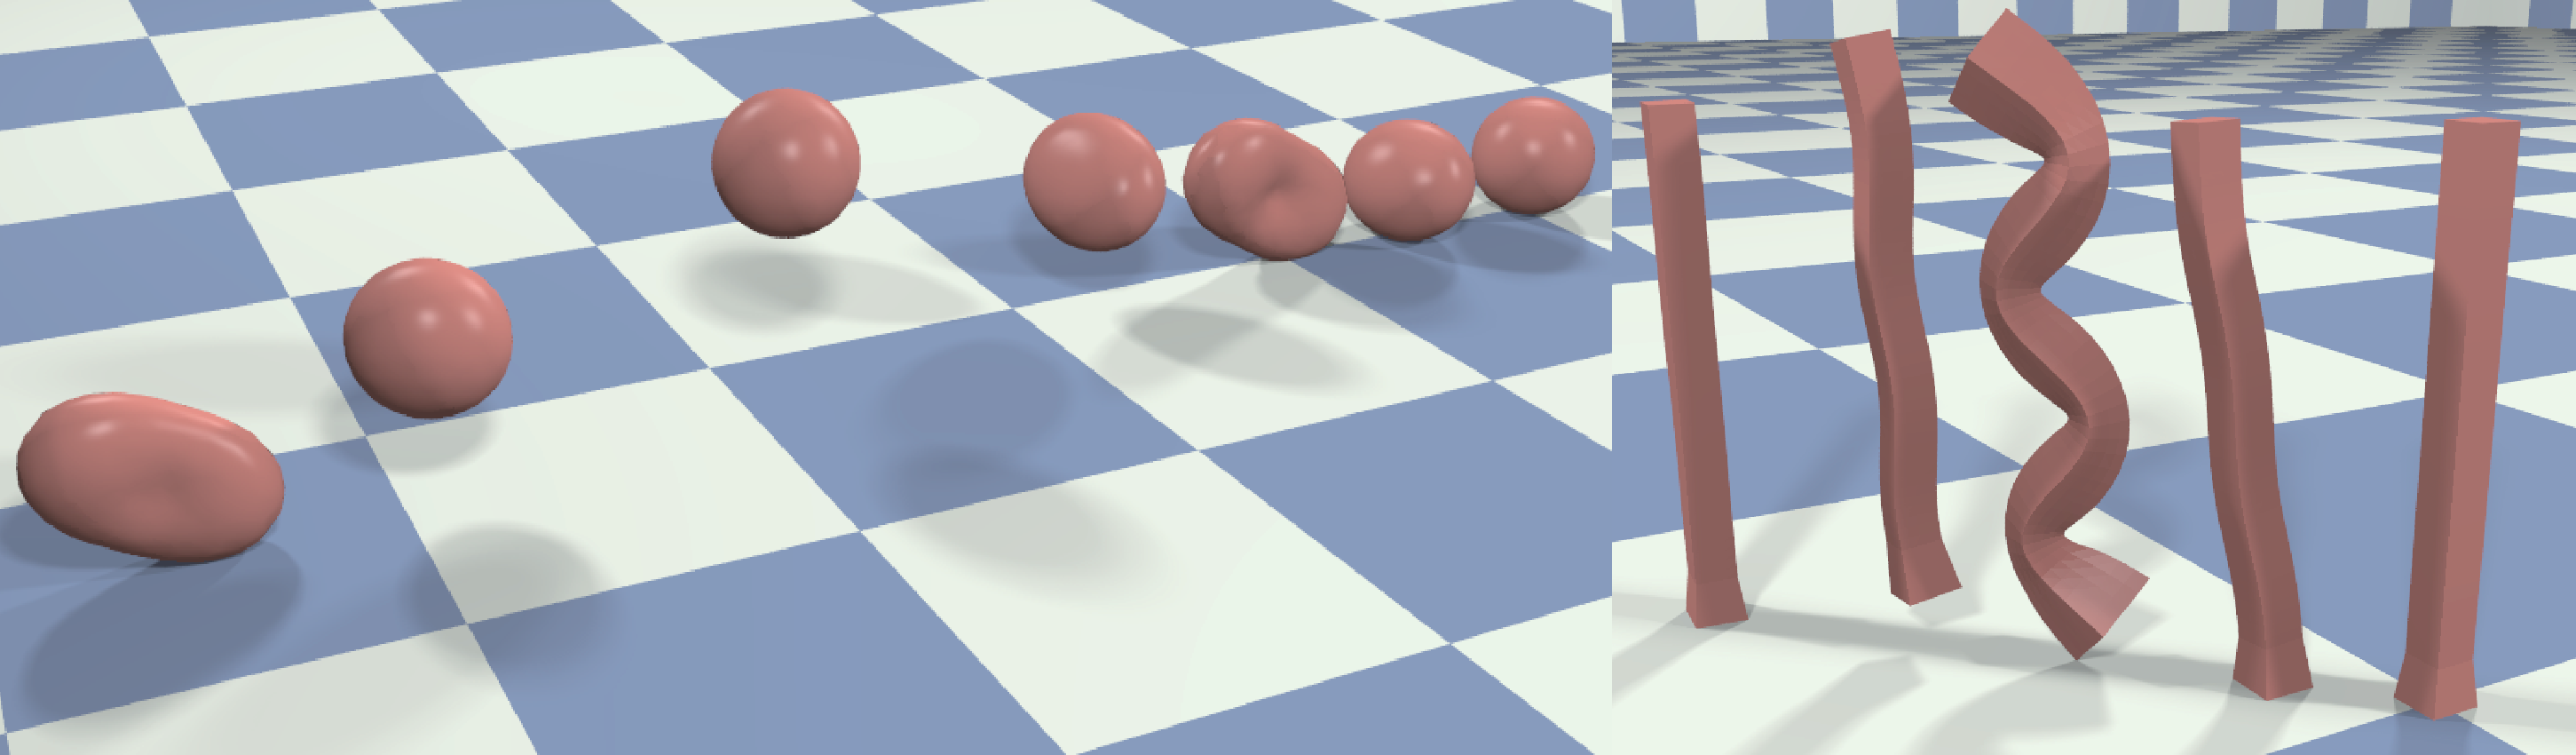
\includegraphics[width=0.99\textwidth]{simulation/defo.pdf}
  \caption{Our novel time-integration scheme \acr{pbdd} can simulate deformable objects such as a ball or a large object with large timesteps for realtime applications.}\label{fig:pbdd}
\end{figure}

Many widely-used deformable body simulation packages are based on implicit time-stepping schemes. These methods model the deformable body's governing equation as an \acr{ode} and then integrate the \acr{ode} using high-order numerical schemes. These methods can be arbitrarily accurate but require small timestep sizes. One simple strategy to improve the runtime performance is to use a large timestep size. This strategy has proven successful in some applications, such as controlling humanoid robots, where the timestep size used in a controller can be larger than that used in the underlying simulator. A key issue in using a large timestep size is ensuring that the time integrator is still stable. For example, the stable region of a semi-implicit Euler integrator shrinks as the timestep size increases. To time integrate a deformable body under a large timestep size, a simple and widely-used method is to use an unconditionally stable fully implicit Euler integrator. However, in a conventional deformable body's governing dynamics equation, the use of a fully implicit Euler integrator involves a costly $\mathcal{O}(N^3)$ computation of high-order derivatives, where $N$ is the number of vertices in a deformable body.

The solver of linear systems in \acr{fem} is used as a sub-system in the simulator. On top of it, the simulator uses a time integration scheme to predict the next configuration. To this end, we develop a time-integration scheme that is stable under large timesteps, as illustrated in \autoref{fig:pbdd}. As a results, less timesteps are needed leading to higher efficiency.  We present \acr{pbdd}, a novel optimization-based algorithm for deformable body dynamics simulation. Unlike prior method, which represents the velocity as a time derivative and evaluates this derivative analytically, our \acr{pbdd} formulation represents this velocity using finite differences in the Euclidean space. This Euclidean space discretization allows us to represent all the physical variables as functions of positions. As a result, we can integrate the system implicitly without high-order derivatives. In addition, we show that numerical simulation under our \acr{pbdd} framework can be recast as a numerical optimization. Therefore, our time integrator is stable under an arbitrarily large timestep size because a numerical optimizer can ensure that the energy value decreases during each iteration through line-search or trust region limitation. Solving these unconstrained minimization problems requires evaluating the energy gradient and/or Hessian and solving a linear system of size $\leq N$ where $N$ is the number of vertices.

\begin{figure}[ht]
  \centering
  \includegraphics[width=0.99\textwidth]{simulation/COMP_Stability.pdf}
  \put(-320,-12){(\emph{a})}
  \put(-200,-12){(\emph{b})}
  \put(-070,-12){(\emph{c})}
  \subcaptionphantom{\label{fig:swing_sim_a}}\vspace{-2ex}
  \subcaptionphantom{\label{fig:swing_sim_b}}\vspace{-2ex}
  \subcaptionphantom{\label{fig:swing_sim_c}}\vspace{-2ex}
  \vspace{-2ex}
  \caption{(\emph{a}) We plot the total kinetic+potential energy over time during a standard simulation of a 10-link chain that swings downward. Each joint of this chain is a 2-DOF ball joint so that this chain has 20-DOF. Forward Euler integrator for the Newton-Euler equation and semi-implicit Euler integrator are not stable. Being fully implicit, our second-order \acr{pbdd} solver is stable but quickly loses energy. By increasing the order by one, both the second-order Runge-Kutta and our third-order \acr{pbdd} solver preserve energy very well. (\emph{b}) For the more challenging task of a 100-link chain (200-DOF) that swings downward, even the second-order Runge-Kutta method is not stable and we have to use the third-order Runge-Kutta method for better energy preservation. Our second-order \acr{pbdd} solver is stable but quickly loses energy. Our third-order \acr{pbdd} solver preserves energy very well. (\emph{c}) We compare the total computational time for generating a \SI{10}{\second} trajectory of a 10-link chain swinging down using a second-order collocation method for \acr{pbdd} and a semi-implicit Euler integrator for a conventional formulation. \acr{pbdd} is 1.5--2.1 times slower at a small timestep size and up to 4 times faster at a large timestep size, such as \SI{0.05}{\second}. The faster time integration is used for real-time rigid and deformable simulation.}\label{fig:swing_sim}
\end{figure}

We compare the accuracy of time integrators for our \acr{pbdd} formulation and conventional formulation. In \autoref{fig:swing_sim_a}, we plot the total kinetic+potential energy over time during a standard simulation of a 10-link chain (20-DOF) that swings downward. The timestep size is \SI{0.0025}{\second}. We can see that \acr{pbdd} is very stable and continuously loses energy (\autoref{fig:swing_sim_a} purple). In contrast, low-order explicit integrators such as forward Euler and semi-implicit Euler are not stable. For better accuracy, we can increase the order of integration by one, resulting in a much better performance in terms of energy preservation. In \autoref{fig:swing_sim_b}, we redo the experiment for a 100-link chain (200-DOF). This is more challenging and low-order explicit integrators are more unstable. The Runge-Kutta method for the Newton-Euler equation is stable at the third order. Although our second-order \acr{pbdd} solver suffers a fast energy loss, increasing the order by one can significantly improve accuracy.

\clearpage%
